% !TeX spellcheck = de_DE

\documentclass{article}

\usepackage[ngerman]{babel}
\usepackage{graphicx}
\usepackage{indentfirst}
\usepackage{hyperref}
\usepackage{geometry}
\usepackage{changepage}
\usepackage{booktabs}
\usepackage{float}
\usepackage{tabulary}
\usepackage{xcolor}
\usepackage{multirow}
\usepackage{caption}
\usepackage{subcaption}
\usepackage{lscape}
\usepackage{colortbl}

\graphicspath{ {./images/} }
\setlength\parindent{0pt}

\hypersetup{
    colorlinks,
    linkcolor={cyan!50!black},
    citecolor={blue!50!black},
    urlcolor={blue!80!black}
}

\makeatletter
\newcommand{\sectionauthor}[1]{
	{\parindent 0em \large \scshape Autor: #1 \par \nobreak \vspace*{1em}}
	\@afterheading
}
\newcommand{\specification}[3]{
	{\parindent 0.5em \hangindent 3em \hypertarget{spec:#1:#2}{\textbf{/#1#2/}} #3 \par \nobreak \vspace*{0.5em}}
}
\makeatother

\title{Bibliotheksanwendung - Feinspezifikation}
\date{\today\\v1.0}
\author{
	Ivan Charviakou\\
	León Liehr\\
	Mohamad Najjar\\
	Jonas Picker\\
	Sergei Pravdin
}

\begin{document}
\maketitle
\begin{figure}[H]
	\centering
	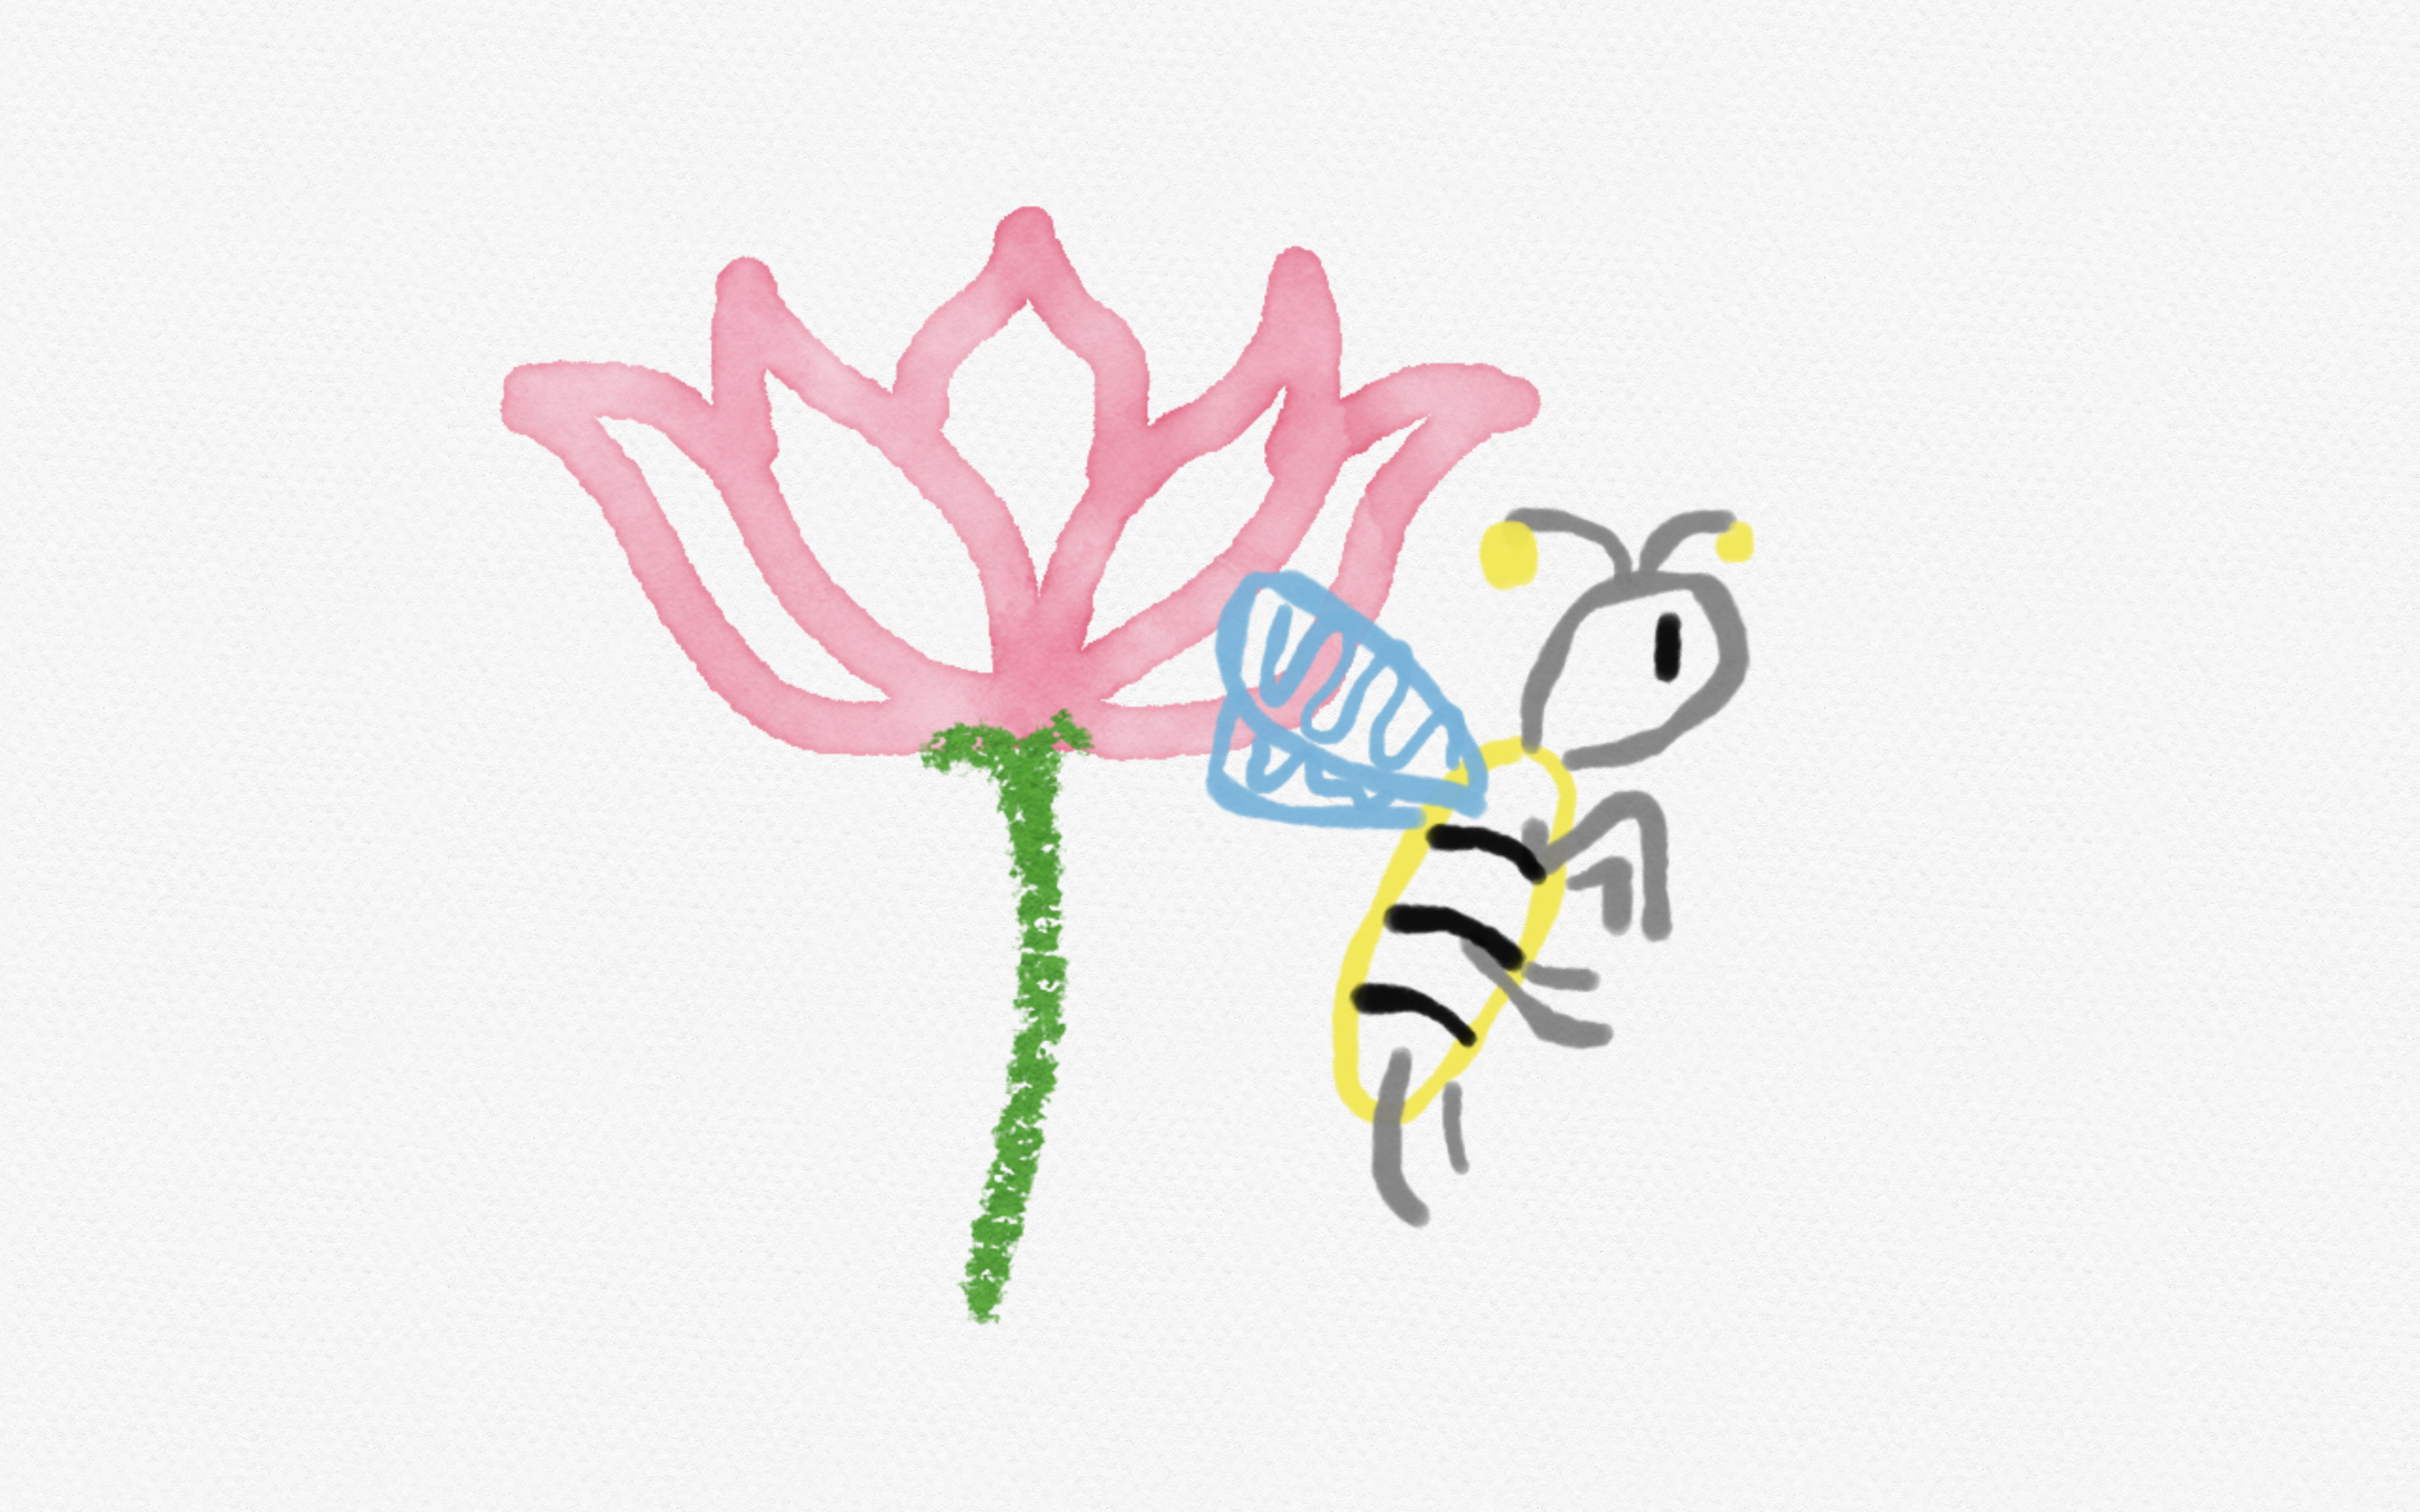
\includegraphics[width = 30em]{Logo}
\end{figure}
\newpage
\tableofcontents
\newpage

%----------------------------------------------------------------------Kapitel 1--------------------------------------------------------------------------------------------

\section{Einleitung}
Bei diesem Dokument handelt es sich um die Feinspezifikation unseres Bibliothekssystems. Es baut direkt auf dem vorangegangenen Entwurf auf und enthält einen noch genaueren Umriss der zu erstellenden Applikation.

%----------------------------------------------------------------------Kapitel 2--------------------------------------------------------------------------------------------

\section{Projektübersicht}
\sectionauthor{Ivan Charviakou}

\subsection{Paketübersicht und Ordnerstruktur}
Das angegebene Diagramm stellt die MVC-Architektur mit den Beziehungen zwischen den einzelnen Komponenten anhand der gegebenen Applikation dar.
Dabei folgt die Komponentenaufteilung der Paketstruktur der Applikation und es werden die Paketnamen zusammen mit den wichtigsten darin enthaltenen Klassen / Komponenten / Funktionalitäten angegeben.
Zudem entsprechen die Farben, die die Pakete im Diagramm besitzen, den Farben im nachfolgenden Klassendiagramm. \vspace{0.5em}

Die Ordnerstruktur des Projekts wird als Ordnerbaum dargestellt.
Während die Paketstruktur im Ordner 'BiBi.src.main.java' abgebildet ist, enthält 'BiBi.src.main.webapp.view' die verwendeten Facelets mit entsprechender Rollenzuordnung. \vspace{0.5em}

\begin{figure}[H]
\centering
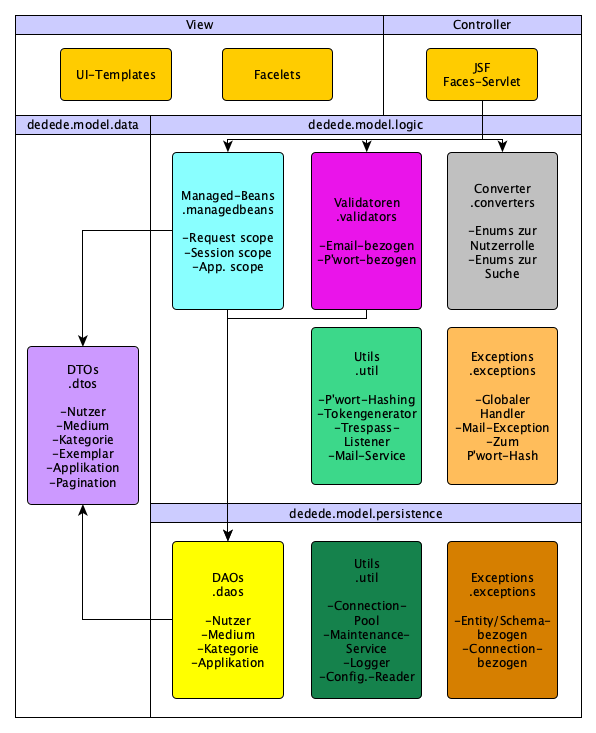
\includegraphics[width = 40em]{Modeldiagramm}
\caption{Modeldiagramm}
\end{figure}

\begin{figure}[H]
\centering
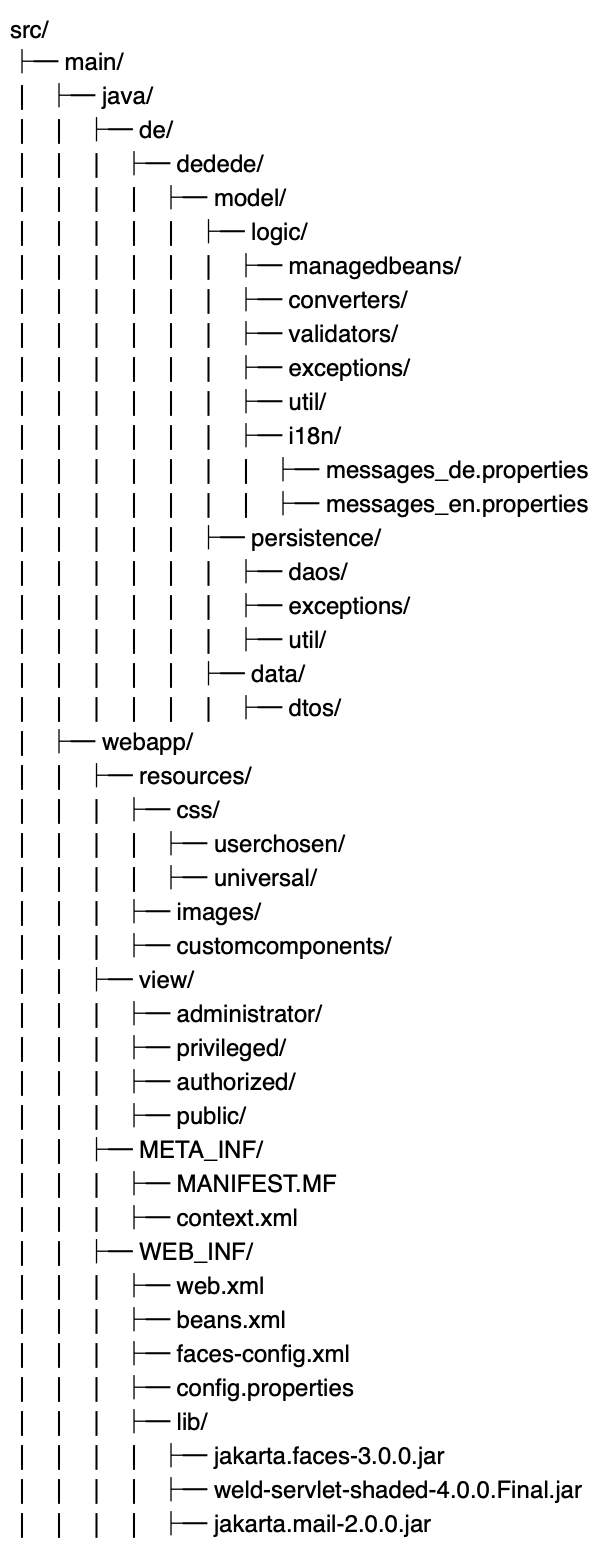
\includegraphics[width = 20em]{FileStructure}
\caption{Ordnerstruktur}
\end{figure}

%----------------------------------------------------------------------Kapitel 3--------------------------------------------------------------------------------------------
\section{UML-Klassendiagramme}
\sectionauthor{Mohamad Najjar}


Das Paketdiagramm veranschaulicht  die Rollen und Beziehungen der Pakete im Sichtmodell. Die Farben der Klassendiagramme entsprechen ihren jeweiligen Paketen im \hyperlink{Pakete}{Paketdiagramm}. Die Kommentare finden sich im Anhang.

\newgeometry{left=0cm,right=0cm,top=0cm,bottom=0cm}
\begin{figure}[H]
\hypertarget{Pakete}
		\centering
		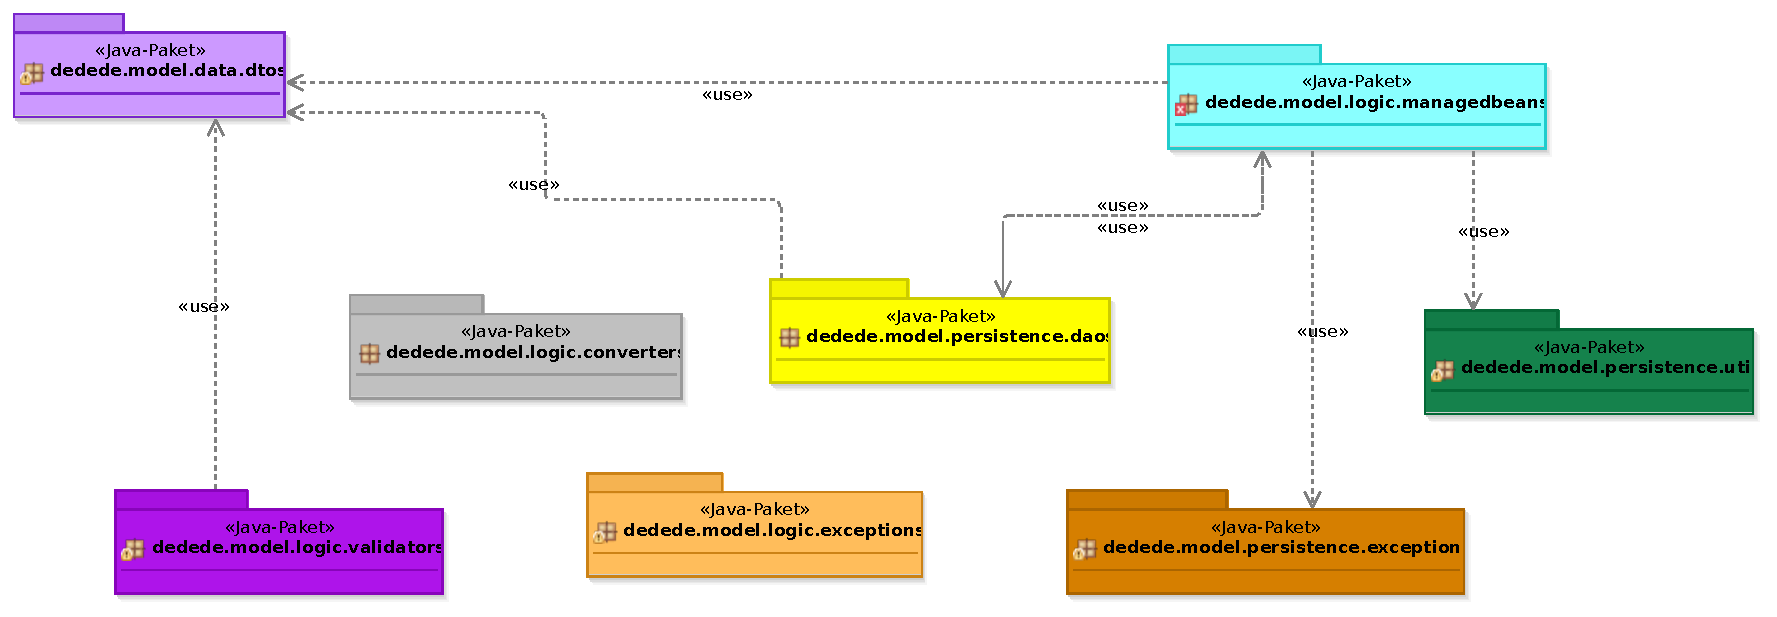
\includegraphics[width = 52em]{Paketdiagramm}
		\caption{Paketdiagramm}
	\end{figure}

\begin{figure}[H]
\hypertarget{DAOs}{}
		\centering
		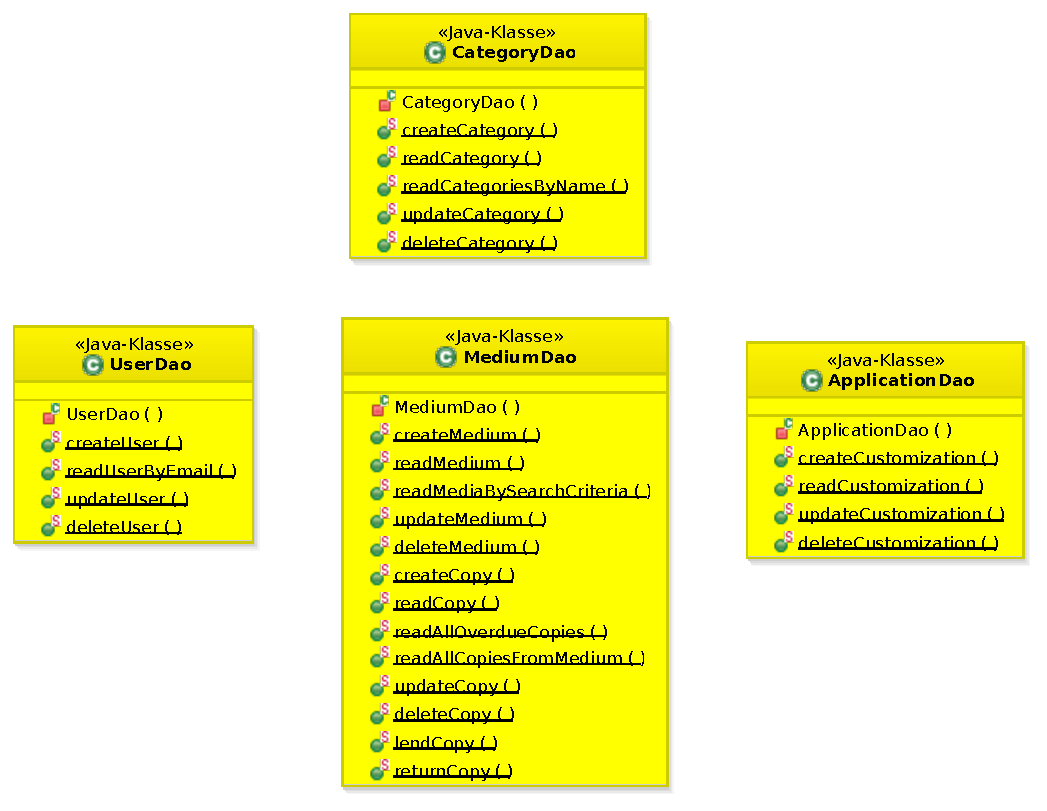
\includegraphics[width = 45em]{KlassendiagrammDaos}
		\caption{Klassendiagramm der Daos}
	\end{figure}

\begin{figure}[H]
\hypertarget{Usersession}{}
		\centering
		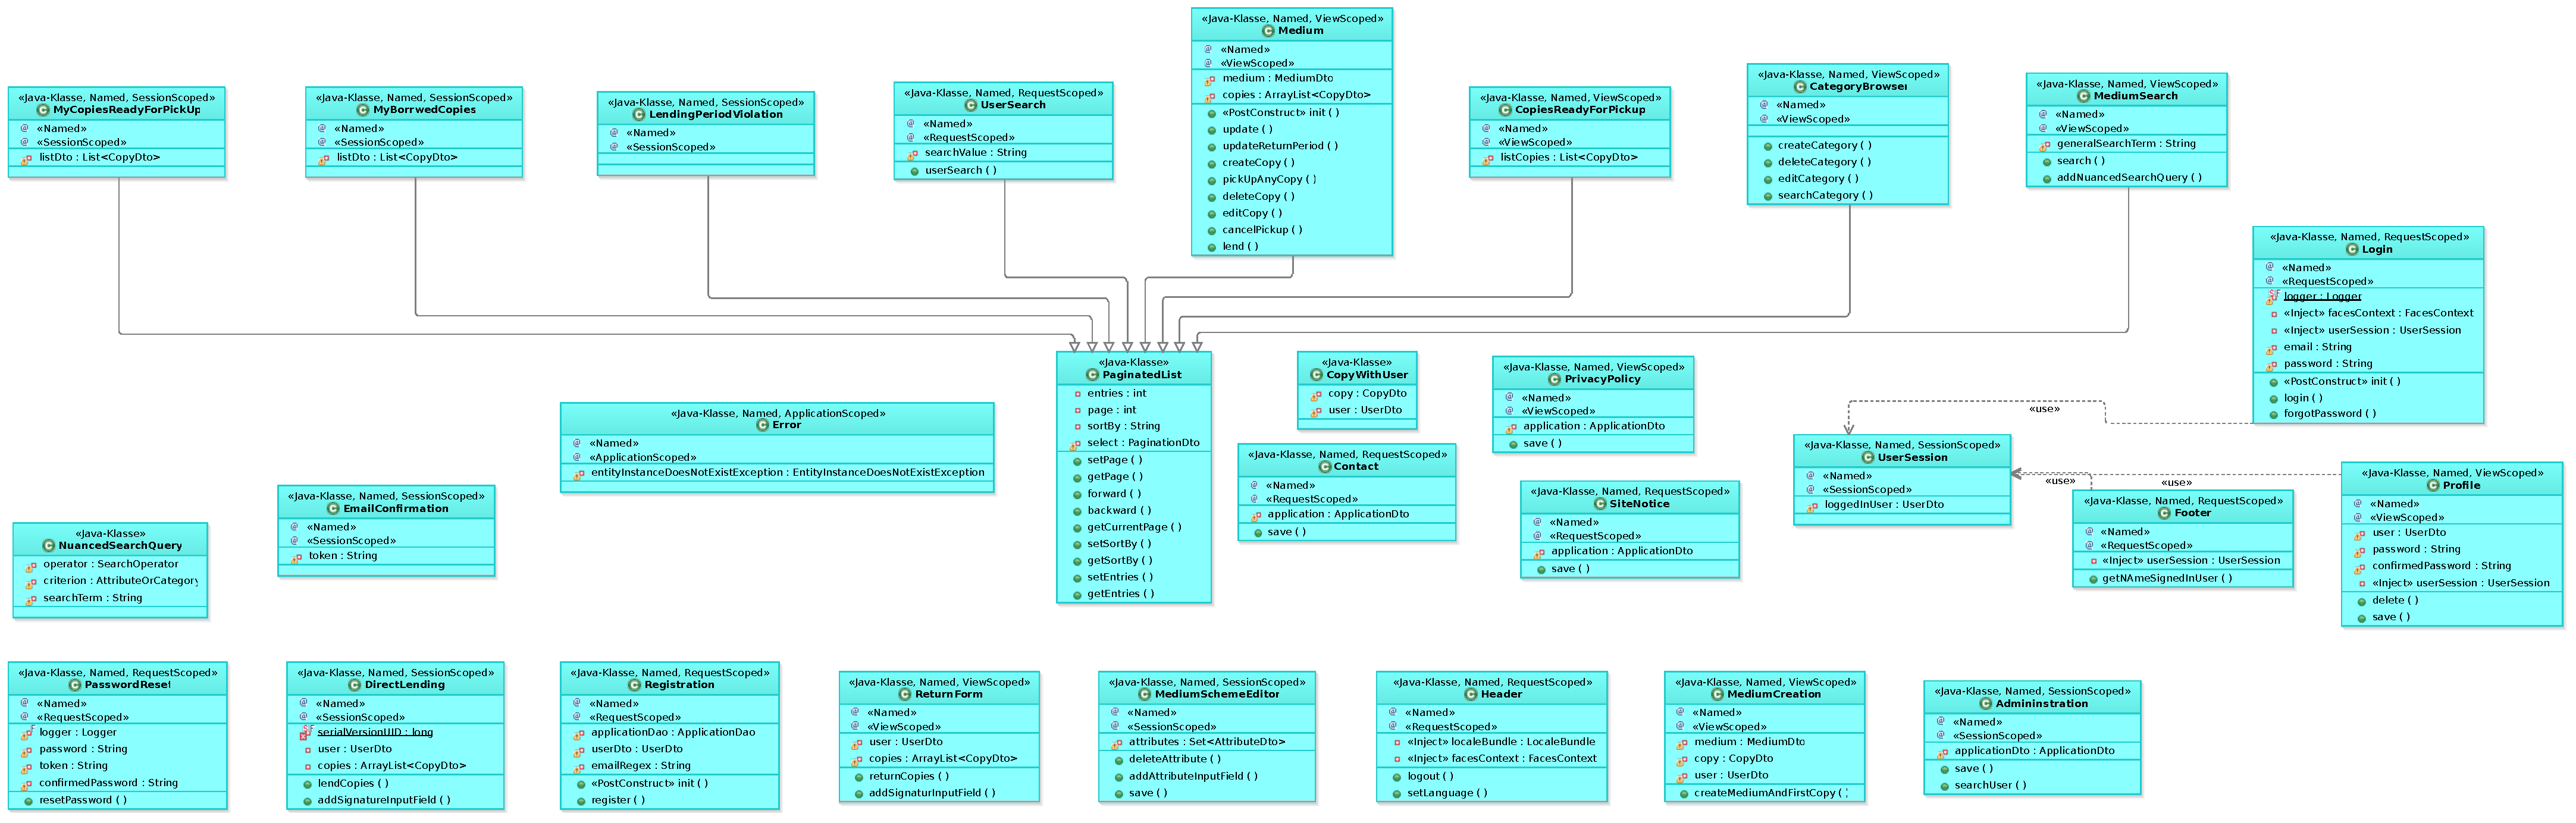
\includegraphics[angle=270, width=24em]{Klassendiagramm-Backingbeans}
		\caption{Klassendiagramm-Backingbeans}
	\end{figure}




\begin{figure}[H]
		\centering
		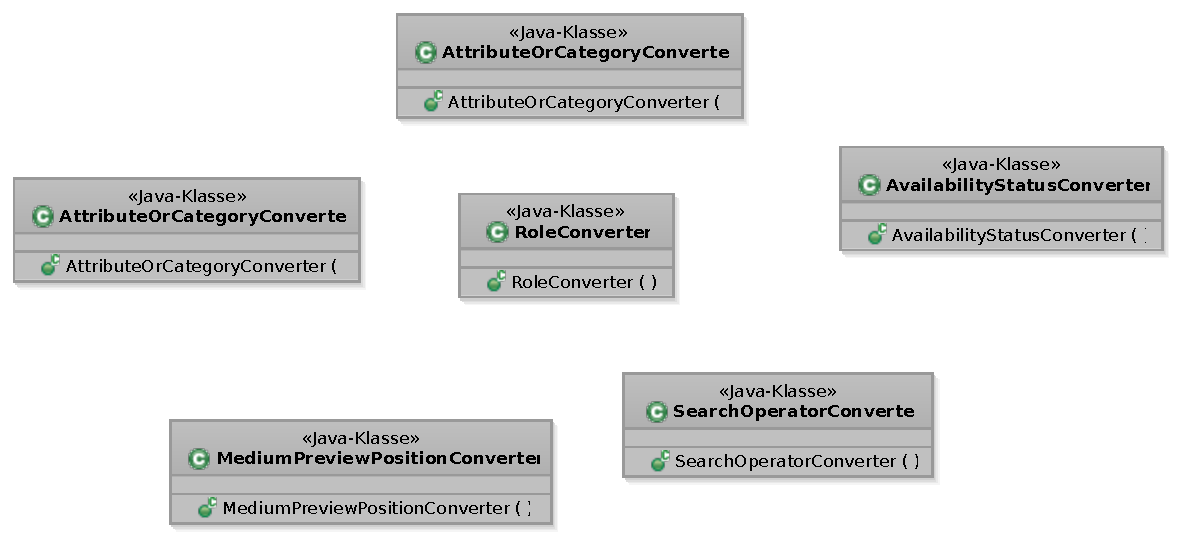
\includegraphics[width = 52em]{Klassendiagramm-Convertors}
		\caption{Klassendiagramm der Konverter}
	\end{figure}

\begin{figure}[H]
\hypertarget{Validator}{}
		\centering
		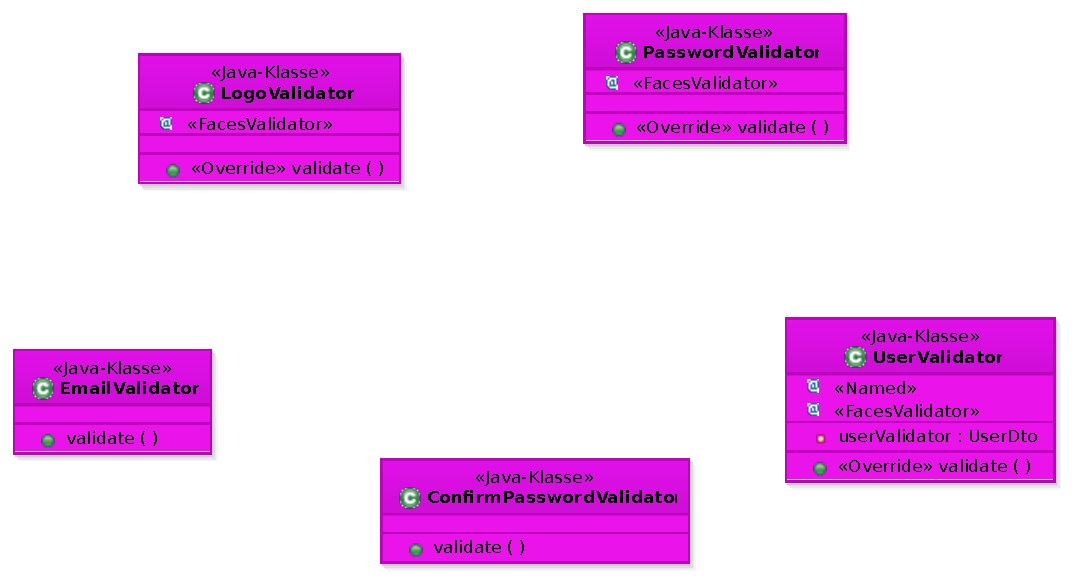
\includegraphics[width = 52em]{KlassendiagrammValidators}
		\caption{Klassendiagramm der Validatoren}
	\end{figure}


\begin{figure}[H]
		\centering
		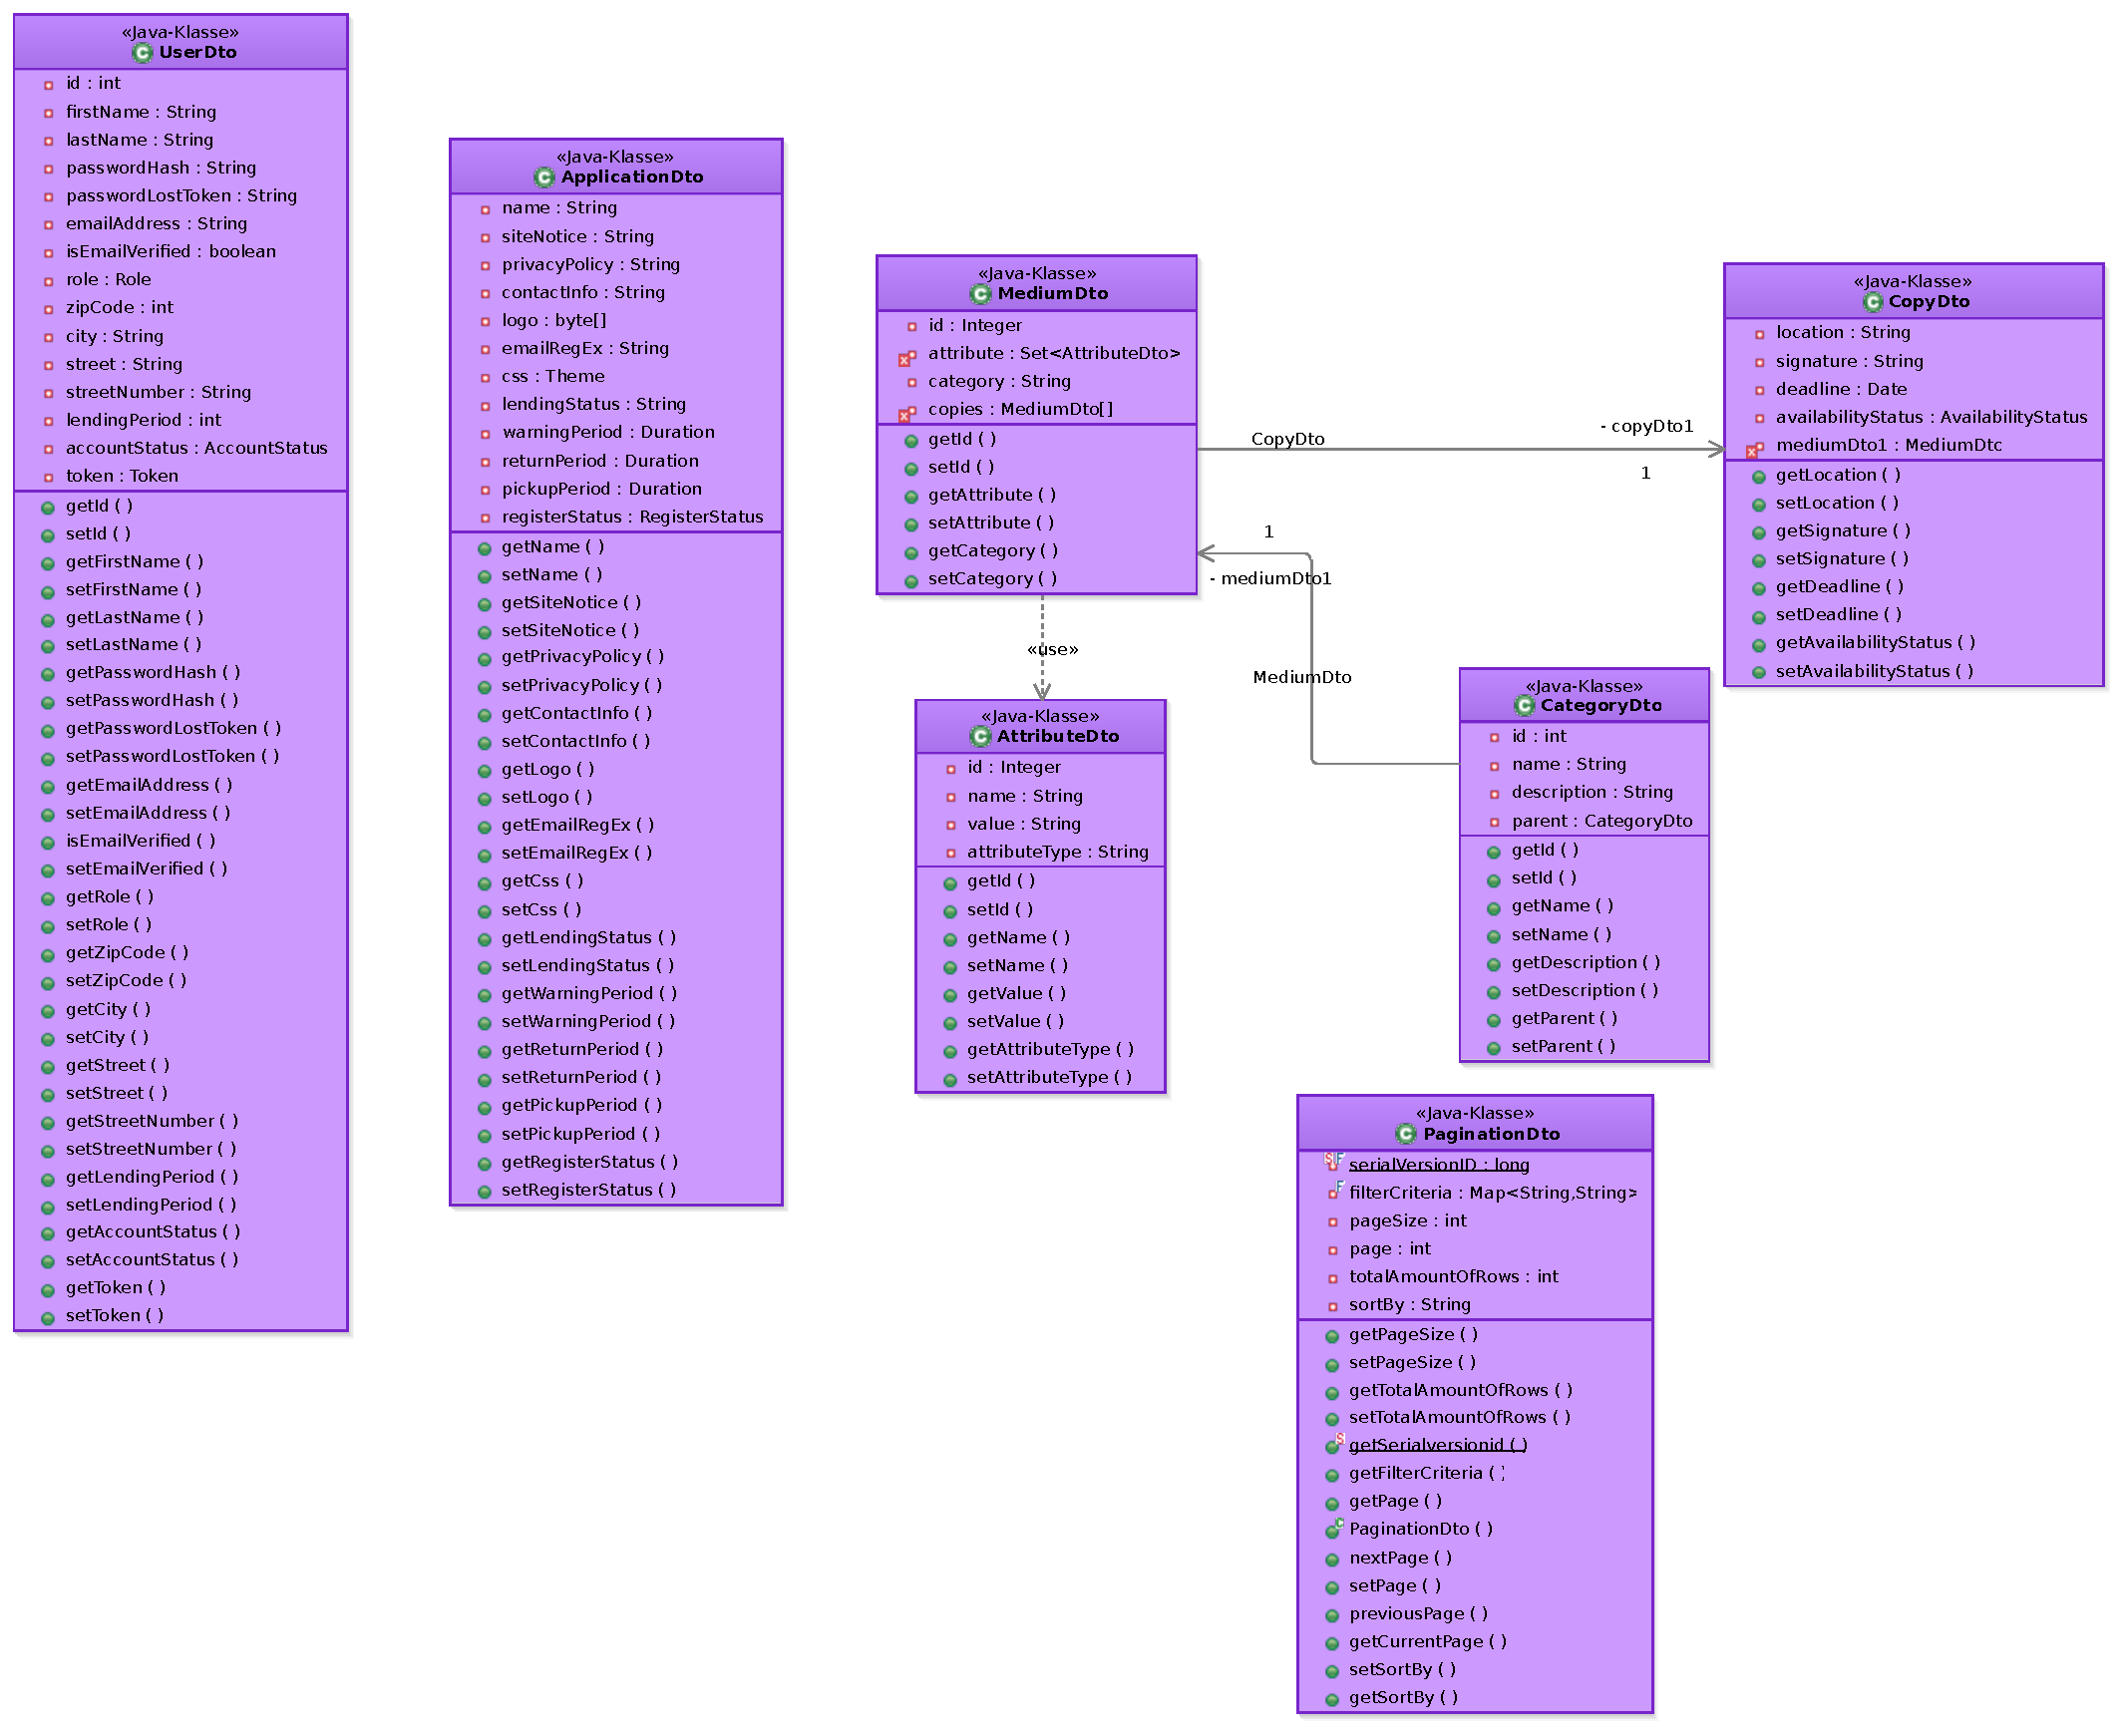
\includegraphics[angle=270, width = 52em]{Klassendiagramm-Dtoss_1}
		\caption{Klassendiagramm der Dtos}
	\end{figure}

\begin{figure}[H]
		\centering
		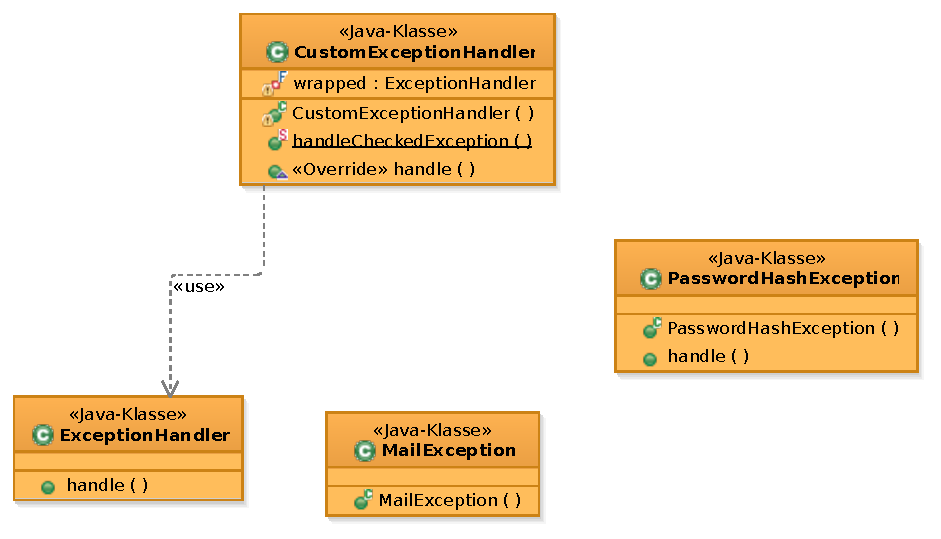
\includegraphics[width = 52em]{Klassendiagramm-ExceptionsObere}
		\caption{Klassendiagramm der logic.exceptions}
	\end{figure}

\begin{figure}[H]
\hypertarget{PhaseListener}{}
\hypertarget{Hash}{}
		\centering
		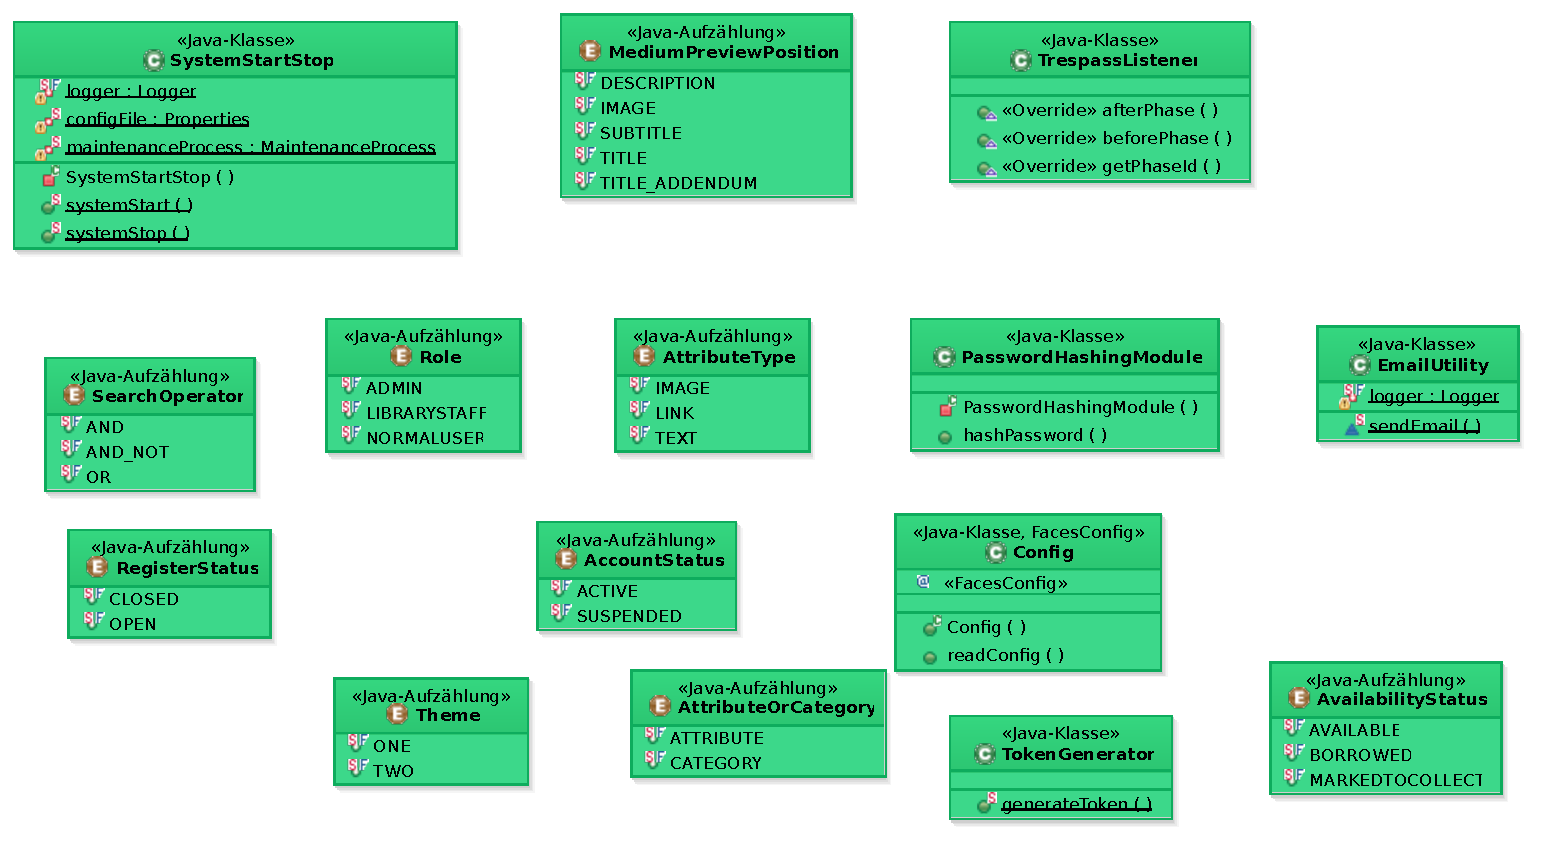
\includegraphics[width = 52em]{KlassendiagrammUtilObere}
		\caption{Klassendiagramm der logic.util}
	\end{figure}


\begin{figure}[H]
		\centering
		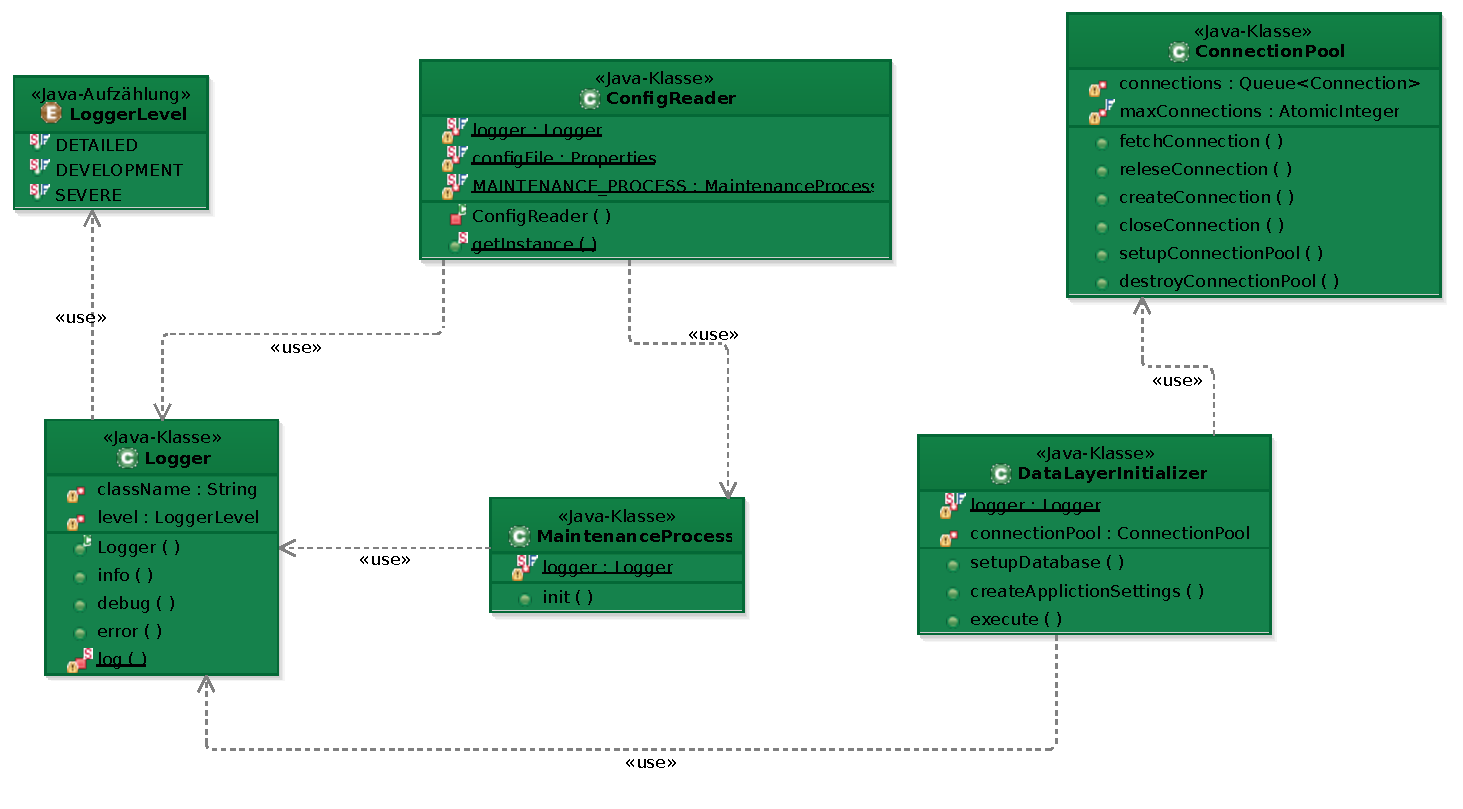
\includegraphics[width = 52em]{KlassendiagrammUtilunten}
		\caption{Klassendiagramm der persistence.util}
	\end{figure}


\begin{figure}[H]
		\centering
		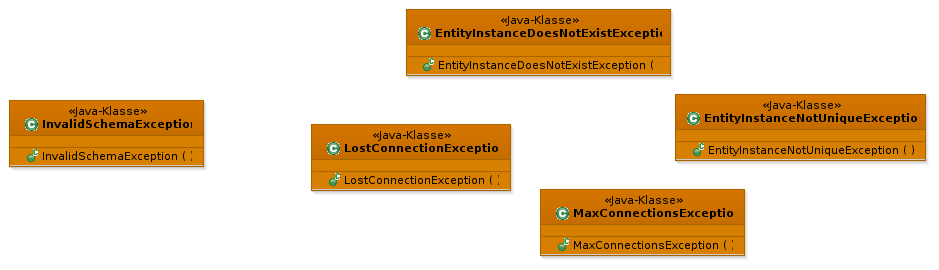
\includegraphics[width = 52em]{Klassendiagramm-ExceptionUnten}
		\caption{Klassendiagramm der persistence.exceptions}
\end{figure}
\restoregeometry
%----------------------------------------------------------------------Kapitel 4--------------------------------------------------------------------------------------------
\newpage
\section{Bibliotheken}
\sectionauthor{Sergei Pravdin}

\newenvironment{controls}
{
    \begin{table}[H]
        \centering
        \begin{tabular}{ p{7em} p{19em} p{4em} p{12em} }
            \toprule
            \textbf{Bibliothek} & \textbf{Anwendungsbereich} & \textbf{Version} & \textbf{Lizenz}\\
            \midrule
        }
        {
            \bottomrule
        \end{tabular}
    \end{table}
}

Folgende Bibliotheken bzw. Frameworks werden für die Entwicklung unseres Bibliothekssystems verwendet.

\begin{controls}
    Jakarta Server Faces (JSF) & Grafische Benutzeroberflächen des Bibliothekssystems & 3.0.0 & GNU GPL / Java Community Process\\
    JDBC-Treiber für PostgreSQL & Integration des Bibliothekssystems mit der Datenbank & 42.2.20 & GNU GPL / Java Community Process\\
    Apache Tomcat & Webserver & 10.0.2 & Apache-Lizenz 2.0\\
    Weld & Dependency Injection mittels Annotationen & 4.0.1 & Apache-Lizenz 2.0\\
    Jakarta Mail & Senden und Empfangen von E-Mails für die Verifizierung der Nutzers & 1.6.5 & CDDL 1.0, GPL 2.0, BSD\\
    Bootstrap & Anordnung der Frontend-CSS-Komponenten & 5.0.0 & MIT-Lizenz\\
\end{controls}

%----------------------------------------------------------------------Kapitel 5--------------------------------------------------------------------------------------------
\section{Systemkonfiguration}
Dieser Abschnitt beschreibt die Konfigurationsdatei und Sprachausgabe der Anwendung.
\subsection{Konfigurationsdatei}
\indent Die Anwendung wird in einer Datei namens 'config' im \hyperlink{https://de.wikipedia.org/wiki/Java-Properties-Datei}{{\texttt.properties}-Format} konfiguriert. Diese Datei wird dann mit Java-internen Funktionalitäten \hyperlink{https://docs.oracle.com/javase/7/docs/api/java/util/Properties.html}{dieser Klasse} über einen Stream eingelesen. Sie ist im Verzeichnis der Anwendung unter \texttt{/WebContent/WEB-INF/} zu finden und ist unten sowohl kurz \hyperlink{configTabelle}{beschrieben}, als auch \hyperlink{configFoto}{fotographiert} .
\subsubsection{Inhaltsbeschreibung}
\hypertarget{propSchema}{}
Die mit \textcolor{green}{!} oder \textcolor{green}{\#} eingeleiteten Zeilen der Dateien enthalten Kommentare. Alle unmarkierten Zeilen halten ein Paar aus einem Schlüssel und einem mit \texttt{:} getrennten Wert. Nur die Werte dürfen verändert werden!

\begin{center}
\begin{table}[H]
\begin{tabular} {| m{4cm} | m{6cm} | m{5cm} |}
\hline
\hypertarget{configTabelle}{Schlüsselname} & Wertebeschreibung & Wertebereich \\
\hline
DB\_HOST & Die URL (bzw. URI) unter der der Datenbankserver erreichbar ist.& Ein \hyperlink{https://datatracker.ietf.org/doc/html/rfc3986}{'Uniform Ressource Identifier'}. Pflichtfeld!\\
\hline
DB\_PORT & Der Port unter dem der Server Anfragen entgegennimmt. & Eine ganze Zahl von 0 bis 65535. Pflichtfeld!\\
\hline
DB\_NAME & Der Name der Datenbank auf dem Server. & Ein String. Pflichtfeld!\\
\hline
DB\_USER & Der Name eines in der Datenbank registrierten Benutzers. & Ein String. Pflichtfeld!\\
\hline
DB\_PASSWORD & Das Passwort des oben angegebenen Datenbankbenutzers. & Ein String. Pflichtfeld!\\
\hline
DB\_CAPACITY & Die maximale Anzahl an Verbindungen, die die Datenbank dem Server zu Verfügung stellen kann. & Eine natürliche Zahl (nicht 0). Standartwert ist 42.\\
\hline
MAILSERVER\_HOST & Der URI unter der der E-Mail-Server erreichbar ist. &  Ein \hyperlink{https://datatracker.ietf.org/doc/html/rfc3986}{'Uniform Ressource Identifier'}. Pflichtfeld! \\
\hline
MAILSERVER\_PORT & Der Port durch den Anfragen an den Server geleitet werden. & Eine ganze Zahl von 0 bis 65535. Pflichtfeld! Standartwert ist 25. \\
\hline
MAIL\_SOURCE & Die Absenderadresse für E-Mails des Bibliothekssystems. & Gültige E-Mail-Adressen folgen \hyperlink{https://datatracker.ietf.org/doc/html/rfc5322}{diesem Schema}. Pflichtfeld!\\
\hline
SCAN\_INTERVAL & Der Wartungsthread des Systems führt in diesem Interval automatische Aufgaben durch. & Eine natürliche Zahl (nicht 0) die Minuten repräsentiert. Standartwert ist 20. \\
\hline
DEFAULT\_ADMIN\_MAIL & Diese Zeichenkette wird ohne Verifizierung als E-Mail des ersten Administratoraccounts eingetragen, falls es noch keinen gibt (im System auch änderbar).  & Gültige E-Mail-Adressen folgen \hyperlink{https://datatracker.ietf.org/doc/html/rfc5322}{diesem Schema}, andernfalls kommen versendete Mails nicht an. Schlüssel ist auch Standartwert.\\
\hline
DEFAULT\_PASSWORD & Das Passwort des obigen Admin-Accounts. Sollte umgehend geändert werden. & Eine (möglichst zufällige) Zeichenkette. Standartwert ist 'bibadmin', dieser sollte sofort geändert werden!. \\
\hline
LOG\_LEVEL & Eine Granularitätsoption für die Protokollierung der Fehler und Systemabläufe. & Im Detailgrad aufsteigend: 'SEVERE', 'DETAILED', 'DEVELOPMENT'. Standart ist 'SEVERE', andere Werte werden ignoriert. \\
\hline
LOG\_CONSOLE & Gibt an, ob die Systemprotokolle auch auf der Konsole ausgegeben oder nur ins Log geschrieben werden. & Ein Boolean aus 'TRUE' oder 'FALSE'. Andere Werte werden ignoriert. Standartwert ist 'FALSE'. \\
\hline
\end{tabular}
\end{table}
\end{center}

\newgeometry{left=0cm,right=0cm,top=0cm,bottom=0cm}
\begin{figure}
\hypertarget{configFoto}{}
\centering
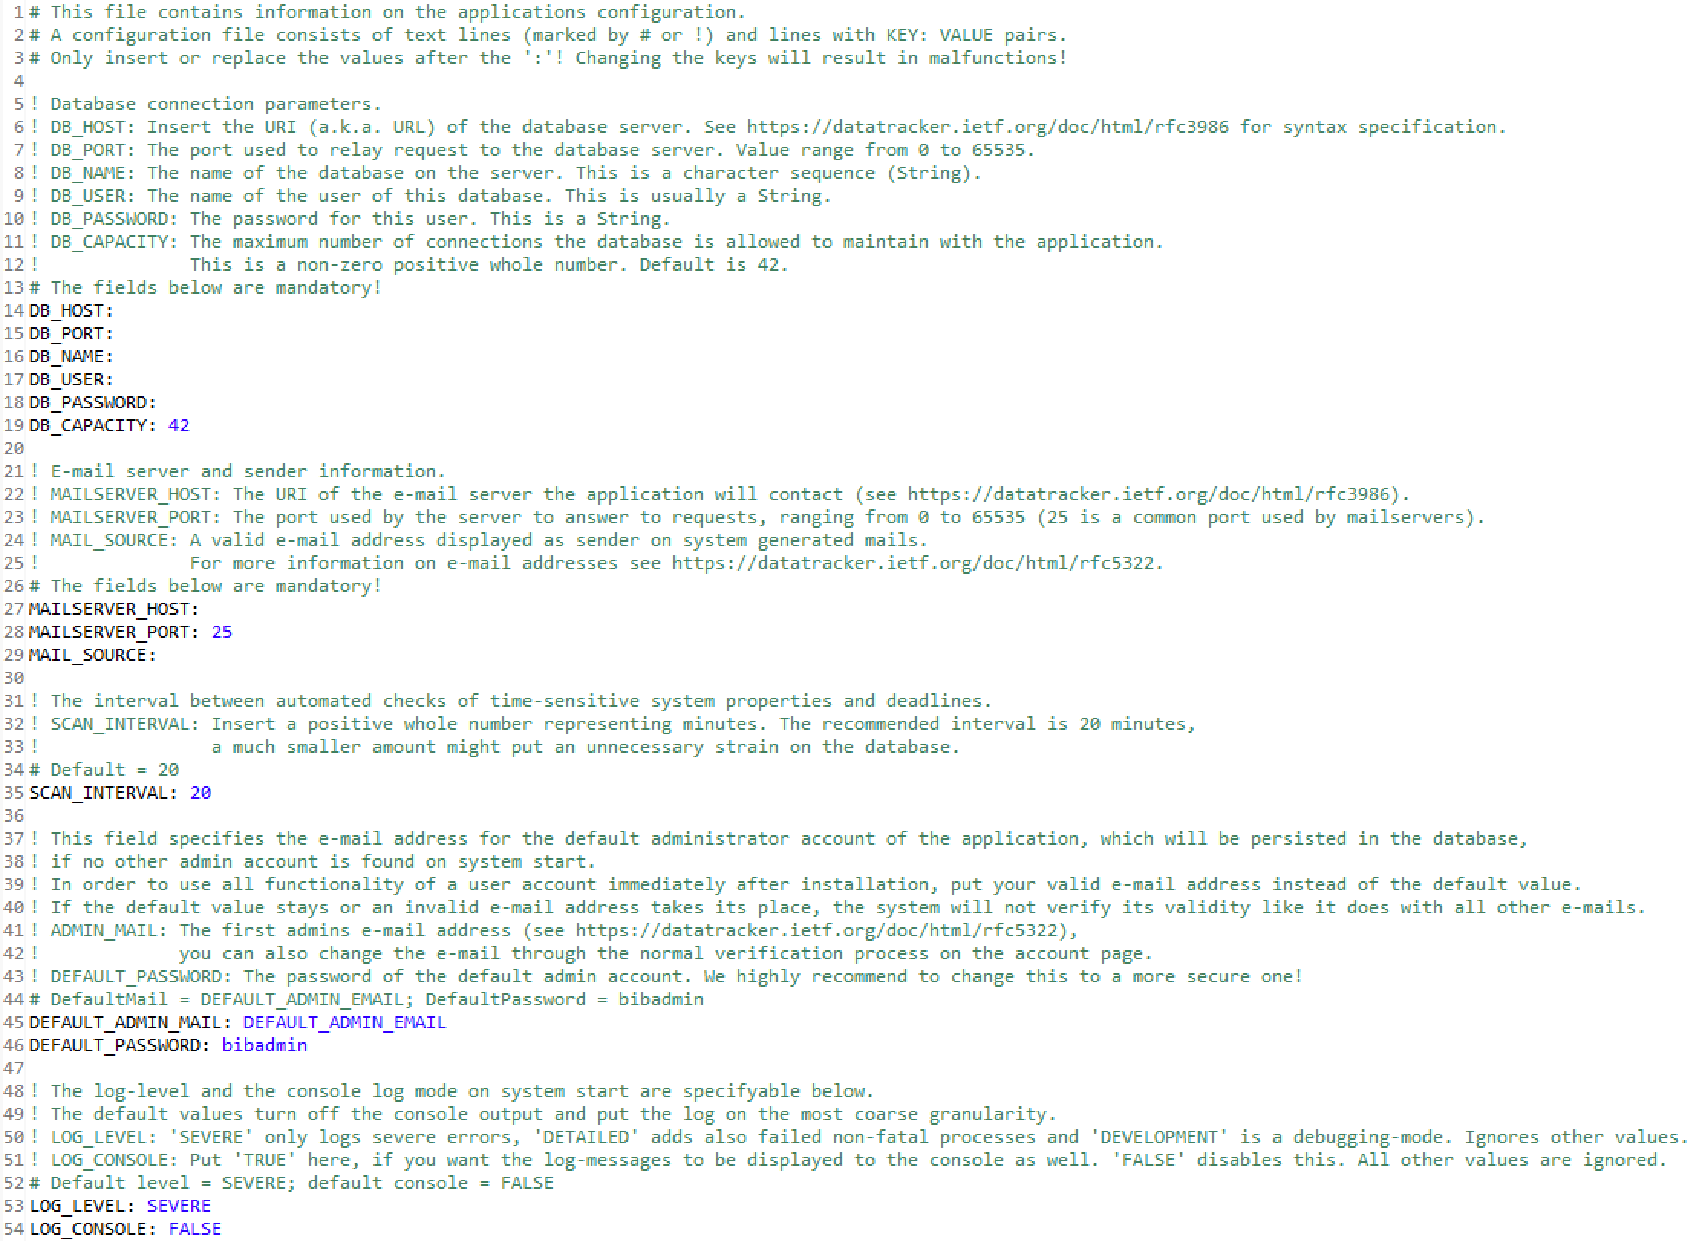
\includegraphics[angle = 270, width = 53em]{configProperties}
\caption{Die \texttt{config.properties} Datei}
\end{figure}
\restoregeometry

\subsection{Sprachressourcen}
\indent Obwohl die Anwendung primär in Deutsch ausgeliefert wird, bietet die modulare Bauweise eine Erweiterungsmöglichkeit um andere Sprachausgaben. Dazu werden alle angezeigten Strings einer Sprache zentral im Ordner \texttt{/src/ressources/} des Applikationsverzeichnisses im \hyperlink{https://de.wikipedia.org/wiki/Java-Properties-Datei}{\texttt{.properties}-Format} gespeichert. Die Namenskonvention für diese Dateien ist \texttt{messages\_xx.properties}, wobei \texttt{xx} durch das jeweilige \hyperlink{https://de.wikipedia.org/wiki/Liste_der_ISO-639-1-Codes}{Sprachenkürzel} ersetzt wird. Die Pakete sind durch Eintrag in die \texttt{faces-config.xml} im JSF-Framework registriert. Damit sind die Schlüssel mittels EL in den Facelets referenzierbar. So kann die Sprache, entweder auf der Profilseite manuell oder auch automatisch durch die Browserpräferenz, pro Nutzer-Session dynamisch eingestellt werden. Standartsprache ist Deutsch. Die Dateien selbst folgen obigen \hyperlink{propSchema}{Schema}. Die Schlüssel können einfach kopiert, mit Werten ergänzt und in den \texttt{/ressources}-Ordner gelegt werden. Ein Beispiel für die \hyperlink{messagesde}{deutsche} und \hyperlink{messagesen}{englische} Datei ist anbei.

\newgeometry{left=0cm,right=0cm,top=0cm,bottom=0cm}
\begin{figure}
\hypertarget{messagesen}{}
\centering
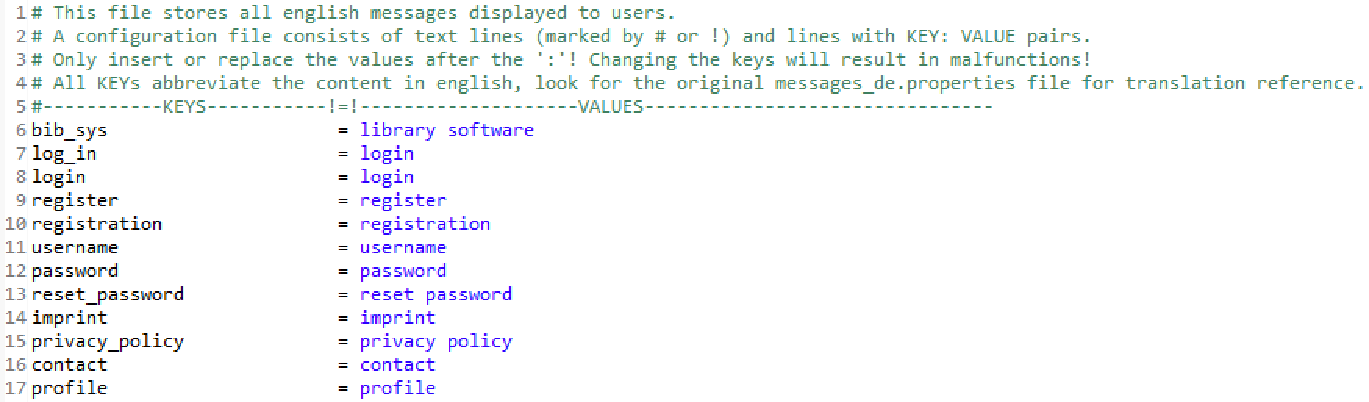
\includegraphics[width=60em]{messagesen}
\caption{Englisches Sprachpaket}
\end{figure}

\begin{figure}
\hypertarget{messagesde}{}
\centering
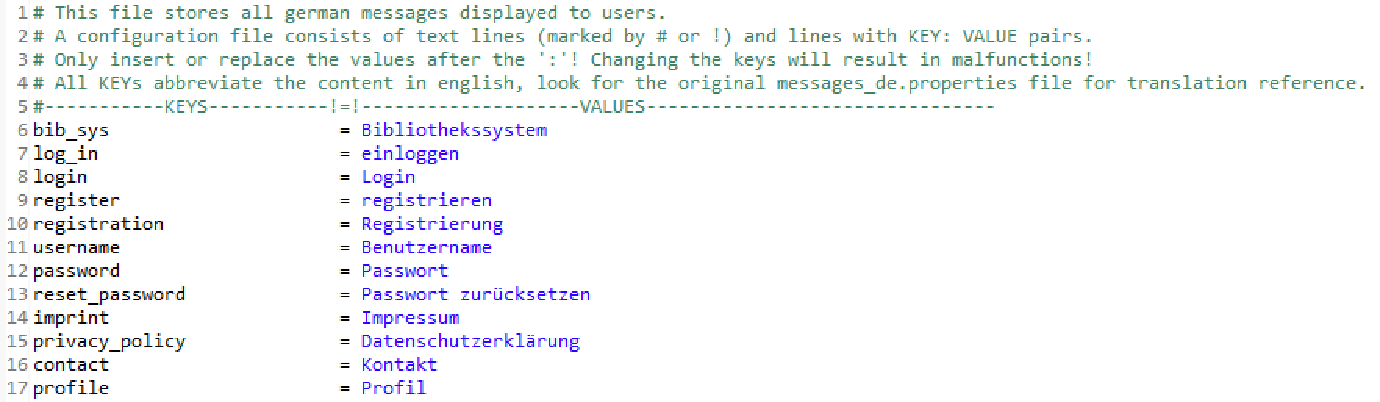
\includegraphics[width=60em]{messagesde}
\caption{Deutsches Sprachpaket}
\end{figure}
\restoregeometry

%----------------------------------------------------------------------Kapitel 6--------------------------------------------------------------------------------------------

\section{View}
\sectionauthor{León Liehr}

\newcommand{\M}[1]{\texttt{#1}} % monospaced
\newcommand{\tag}[2]{\M{#1:#2}} % JSF tag
\newcommand{\B}[1]{\M{\RB{#1}}} % (monospaced) JSF binding
\newcommand{\RB}[1]{\#\{#1\}} % non-monospaced ("raw") JSF binding
\newcommand{\2}[1]{\multirow{2}{*}{#1}}
\newcommand{\3}[1]{\multirow{3}{*}{#1}}
\definecolor{lightgray}{rgb}{0.9,0.9,0.9}
\newcommand{\disambiguationrule}{\arrayrulecolor{lightgray}\cmidrule(r){3-4}\arrayrulecolor{black}}
\newcommand{\INDENT}{\hspace{0.3cm}}

\long\def\begincontrols [#1] #2\endcontrols
{
    \begin{table}[H]
        \centering
        \begin{tabular}{ l l l l }
            \toprule
            & & \multicolumn{2}{l}{\textbf{Attribut}}\\
            \cmidrule(r){3-4}
            \textbf{Tag} & \textbf{Beschreibung} & \textbf{Name} & \textbf{Bindung}\\
            \midrule
            #2
            \bottomrule
        \end{tabular}
        \caption{Bedienelemente in \M{#1.xhtml}}
    \end{table}
}

\long\def\beginsubcontrols [#1][#2] #3\endsubcontrols
{
    \begin{table}[H]
        \centering
        \begin{tabular}{ l l l l }
            \toprule
            & & \multicolumn{2}{l}{\textbf{Attribut}}\\
            \cmidrule(r){3-4}
            \textbf{Tag} & \textbf{Beschreibung} & \textbf{Name} & \textbf{Bindung}\\
            \midrule
            #3
            \bottomrule
        \end{tabular}
        \caption{Bedienelemente pro #1}
        \label{#2}
    \end{table}
}

\newcommand{\component}[2]{\subsubsection{#1 (\texttt{#2})}}

\newcommand{\BTN}{\tag{h}{commandButton}}
\newcommand{\LNK}{\tag{h}{outputLink}}
\newcommand{\INP}{\tag{h}{inputText}}
\newcommand{\PAS}{\tag{h}{inputSecret}}
\newcommand{\DRP}{\tag{h}{selectOneMenu}}
\newcommand{\CHK}{\tag{h}{selectBooleanCheckbox}}
\newcommand{\OUT}{\tag{h}{outputText}}
\newcommand{\LST}{\tag{bibi}{paginatedList}}
\newcommand{\TXT}{\tag{h}{inputTextarea}}
\newcommand{\PRM}{\tag{f}{viewParam}}
\newcommand{\FRM}{\tag{h}{form}}

Was noch fehlt:

% question evtl h:link instead of h:outputLink for links with query params??

\begin{itemize}
    \item (IDs pro Element)
    \item Composite-Component-Definition von paginierten Listen
    \item Composite-Component-Definition von paginierten Baumansichten
    \item Composite-Component-Definition von reaktiven Eingabefeldern
    \item Drop-Down-Listen werden noch nicht befüllt (mit Strings aus dem LocaleBundle)
    \tag{ui}{repeat} \tag{f}{selectItem}
    \item Converters und Validators sind nicht aufgezeichnnet
    \item Verifiziert, dass alle input-felder form-felder haben
    \item \M{MediumSearchDTO} etc
\end{itemize}

\begin{table}[H]
    \centering
    \begin{tabular}{ l l }
        \toprule
        \textbf{Präfix} & \textbf{URI} \\
        \midrule
        \M{bibi} & http://xmlns.jcp.org/jsf/composite/bibi \\
        \M{cc} & http://xmlns.jcp.org/jsf/composite \\
        \M{f} & http://xmlns.jcp.org/jsf/core \\
        \M{h} & http://xmlns.jcp.org/jsf/html \\
        \M{ui} & http://xmlns.jcp.org/jsf/facelets \\
        \bottomrule
    \end{tabular}
    \caption{Verwendete XML-Namensräume}
\end{table}

Jedes \PRM-Element ist in ein \tag{f}{metadata}-Element eingebettet.
META TASK implizit jedes Eingabefeld von Meldungsfeld begleitet.
META NOTE Typ ist JSF-Tag.

% TASK forms

\newgeometry{left=0.5cm,right=0.5cm,top=0cm,bottom=2cm}
\begin{landscape}

\subsection{Komponenten}

JSF Composite Components.

\subsection{Seitenvorlage}\label{page_template}

JSF Templates.

\begincontrols[template]
    \tag{ui}{insert} & Titel einer Seite & \M{name} & \M{title}\\
    \tag{ui}{insert} & Inhalt einer Seite & \M{name} & \M{content}\\
    \tag{ui}{include} & Kopfzeile jeder Seite & \M{src} & \hyperref[page_header]{\M{header.xhtml}}\\
    \tag{h}{messages} & allgemeine Meldungen & \M{globalOnly} & \M{true}\\
    \tag{ui}{include} & Fußzeile jeder Seite & \M{src} & \hyperref[page_footer]{\M{footer.xhtml}}\\
\endcontrols

\subsubsection{Kopfzeile}\label{page_header}

\begincontrols[header]
    \BTN & kontextsensitive Hilfe anzeigen & \M{action} & \B{header.displayHelpText()}\\
    % BEACON TASK + rendered=header.shouldShowHelpText
    \OUT & kontextsensitive Hilfe & \M{value} & BUNDLE-HELP\\
    \FRM & & &\\
    \INDENT\INP & Mediensuchterm & \M{value} & \B{header.mediumSearchTerm} \\ % BEACON store in sep DTO
    \LNK & zur erweiterten Suche & \M{value} & \hyperref[page_medium_search]{\M{public/medium-search.xhtml}}\\
    \tag{h}{graphicImage} & Logo des Systems & \M{value} & \B{header.application.logo}\\
    \OUT & Name des Systems & \M{value} & \B{header.application.name}\\
    \FRM & & \M{rendered} & \B{session.user != null}\\
    \INDENT\tag{h}{commandLink} & abmelden & \M{action} & \B{header.logOut()}\\
    \disambiguationrule
    \2{\LNK} & \2{zur Anmeldemaske} & \M{value} & \hyperref[page_login]{\M{public/login.xhtml}}\\
    & & \M{rendered} & \B{session.user == null}\\
    \disambiguationrule
    \2{\LNK} & \2{zur Registrierungsseite} & \M{value} & \hyperref[page_registration]{\M{public/registration.xhtml}}\\
    & & \M{rendered} & \B{session.user == null}\\
    \disambiguationrule
    \2{\LNK} & \2{zur Profilseite} & \M{value} & \hyperref[page_profile]{\M{account/profile.xhtml?id=\RB{session.user.id}}}\\
    & & \M{rendered} & \B{session.user != null}\\
    \disambiguationrule
    \2{\LNK} & \2{zur Direktausleihe} & \M{value} & \hyperref[page_direct_lending]{\M{staff/direct-lending.xhtml}}\\
    & & \M{rendered} & \B{session.user.role >= 'STAFF'}\\
    \disambiguationrule
    \2{\LNK} & \2{zur Medienrückgabe} & \M{value} & \hyperref[page_return_form]{\M{staff/return-form.xhtml}}\\
    & & \M{rendered} & \B{session.user.role >= 'STAFF'}\\
    \disambiguationrule
    \2{\LNK} & \2{zu den abzuholenden Exemplaren aller Nutzer} & \M{value} & \hyperref[page_copies_ready_for_pickup_all_users]{\M{staff/copies-ready-for-pickup-all-users.xhtml}}\\
    & & \M{rendered} & \B{session.user.role >= 'STAFF'}\\
    \disambiguationrule
    \2{\LNK} & \2{zur Medienerstellung} & \M{value} & \hyperref[page_medium_creator]{\M{staff/medium-creator.xhtml}}\\
    & & \M{rendered} & \B{session.user.role >= 'STAFF'}\\
\endcontrols

\subsubsection{Fußzeile}\label{page_footer}

\begincontrols[footer]
    \LNK & zur Datenschutzerklärung & \M{value} & \hyperref[page_privacy_policy]{\M{public/privacy-policy.xhtml}}\\
    \LNK & zum Impressum & \M{value} & \hyperref[page_site_notice]{\M{public/site-notice.xhtml}}\\
    \LNK & zur Kontaktseite & \M{value} & \hyperref[page_contact]{\M{public/contact.xhtml}}\\
\endcontrols

\subsection{Seiten}

% QUESTION can we replace this???
\subsubsection{Abzuholende Exemplare aller Nutzer}\label{page_copies_ready_for_pickup_all_users}

\begincontrols[staff/copies-ready-for-pickup-all-users]
    \LST & abzuholende Exemplare & &\\
\endcontrols

% !!!!!!!!!! TASK USE SUBCONTROLS
%\begin{table}[H]
%    \centering
%    \begin{tabular}{ p{6em} p{6em} p{19em} p{7em} }
%        \toprule
%        \textbf{Spalte} & \textbf{Tag} & \textbf{Beschreibung} & \textbf{Sichtbarkeit}\\
%        \midrule
%        Exemplar & \LNK & die Signatur eines Exemplars; zur Direktausleihe & \BIB\\
%        Medium & \LNK & Medienattribut mit der Medienvorschauposition Titel; zur Mediensansicht & \BIB\\
%        Nutzer & \OUT & E-Mail-Adresse & Nicht-\ADM\\
%        Nutzer & \LNK & E-Mail-Adresse; zum Profil & \ADM\\
%        Zeit & \OUT & Dauer bis zum Zeitpunkt der Fristüberschreitung & \BIB\\
%        \bottomrule
%    \end{tabular}
%    \caption{Inhalt der paginierten Liste. Jede Zeile existiert pro Exemplar und Nutzer}
%\end{table}

\subsubsection{Abzuholende Exemplare}\label{page_copies_ready_for_pickup}

\begincontrols[account/copies-ready-for-pickup]
    \3{\PRM} & \3{Kennzeichen des Nutzers} & \M{name} & \M{id}\\
    & & \M{value} & \B{copiesReadForPickup.user}\\
    & & \M{required} & \M{true}\\ % QUESTION ooor show for all users if missing??
    \disambiguationrule
    \LST & aller abzuholenden Exemplare & &\\
\endcontrols

% !!!!!!!!!!!!!!! TASK USE SUBCONTROLS
\begin{table}[H]
    \centering
    \begin{tabular}{ p{6em} p{6em} p{27em} }
        \toprule
        \textbf{Spalte} & \textbf{Tag} & \textbf{Beschreibung}\\
        \midrule
        Exemplar & \OUT & die Signatur eines Exemplars\\
        Medium & \LNK & Medienattribut mit der Medienvorschauposition Titel; zur Mediensansicht\\
        Zeit & \OUT & Dauer bis zum Überschreiten der Abholungsfrist\\
        \bottomrule
    \end{tabular}
    \caption{Inhalt der paginierten Liste. Jede Zeile existiert pro Exemplar}
\end{table}

\subsubsection{Ausgeliehene Exemplare}\label{page_borrowed_copies}

\begincontrols[account/borrowed-copies]
    \3{\PRM} & \3{Kennzeichen des Nutzers} & \M{name} & \M{id}\\
    & & \M{value} & \B{myBorrowedCopies.user}\\
    & & \M{required} & \M{true}\\ % QUESTION ooor show for all users if missing??
    \disambiguationrule
    \LST & aller ausgeliehenen Exemplare & &\\
\endcontrols

% !!!!!!!!!!!!!!!!!!!! TASK USE SUBCONTROLS
\begin{table}[H]
    \centering
    \begin{tabular}{ p{6em} p{6em} p{27em} }
        \toprule
        \textbf{Spalte} & \textbf{Tag} & \textbf{Beschreibung}\\
        \midrule
        Exemplar & \OUT & die Signatur eines Exemplars\\
        Medium & \LNK & Medienattribut mit der Medienvorschauposition Titel; zur Mediensansicht\\
        Zeit & \OUT & Dauer bis zum Überschreiten der Rückgabefrist\\
        \bottomrule
    \end{tabular}
    \caption{Inhalt der paginierten Liste. Jede Zeile existiert pro Exemplar}
\end{table}

\subsubsection{Anmeldemaske}\label{page_login}

\begincontrols[public/login]
    \OUT & & \M{rendered} & \B{session.user != null} \\ % TASK note that you are already logged in
    \FRM & & \M{rendered} & \B{session.user == null}\\
    \INDENT\INP & E-Mail-Adresse & \M{value} & \B{login.user.emailAddress}\\
    \INDENT\PAS & Passwort & \M{value} & \B{login.password} \\ % BEACON password converter to hash
    \INDENT\BTN & anmelden & \M{action} & \B{login.logIn()}\\
    \INDENT\tag{h}{commandLink} & Passwort zurücksetzen & \M{action} & \B{login.resetPassword()}\\
\endcontrols

\subsubsection{Datenschutzerklärung}\label{page_privacy_policy}

\begincontrols[public/privacy-policy]
    \FRM & & &\\
    \disambiguationrule
    \INDENT\2{\TXT} & \2{Datenschutzerklärung} & \M{value} & \B{privacyPolicy.application.privacyPolicy}\\
    & & \M{readonly} & \B{session.user.role < 'ADMIN'}\\
    \disambiguationrule
    \INDENT\2{\BTN} & \2{Änderungen speichern} & \M{action} & \B{privacyPolicy.save()}\\
    & & \M{rendered} & \B{session.user.role == 'ADMIN'}\\
\endcontrols

\subsubsection{Direktausleihe}\label{page_direct_lending}

\begincontrols[staff/direct-lending]
    \tag{bibi}{reactiveInputText} & E-Mail-Adresse des Kunden & \M{value} & \B{directLending.user.emailAddress}\\
    \disambiguationrule
    \2{\tag{ui}{repeat}} & \2{Signaturen der auszuleihenden Exemplare} & \M{value} & \B{directLending.copies}\\
    & & \M{var} & \hyperref[subcontrol_direct_lending_copy]{\M{copy}}\\
    \disambiguationrule
    \BTN & weiteres Signatureingabefeld hinzufügen & \M{action} & \B{directLending.addSignatureInputField()}\\
    \BTN & Exemplare verleihen & \M{action} & \B{directLending.lendCopies()}\\
\endcontrols

\beginsubcontrols[Exemplar (5 bei Seitenaufruf)][subcontrol_direct_lending_copy]
\tag{bibi}{reactiveInputText} & Signatur des Exemplars & \M{value} & \B{copy.signature}\\
\endsubcontrols

\subsubsection{E-Mail-Bestätigung}\label{page_email_confirmation}

\begincontrols[public/email-confirmation]
    \3{\PRM} & \3{Kennzeichen der E-Mail-Bestätigung} & \M{name} & \M{token}\\
    & & \M{value} & \B{emailConfirmation.token}\\
    & & \M{required} & \M{true}\\
\endcontrols

\subsubsection{Fehlerseite}\label{page_error}

% BEACON TASK from where do we get the information?

\begincontrols[public/error]
    \OUT & ?? & &\\
\endcontrols

\subsubsection{Impressum}\label{page_site_notice}

\begincontrols[public/site-notice]
    \FRM & & &\\
    \disambiguationrule
    \INDENT \2{\TXT} & \2{Impressum} & \M{value} & \B{siteNotice.application.siteNotice}\\
    & & \M{readonly} & \B{session.user.role < 'ADMIN'}\\
    \disambiguationrule
    \INDENT\2{\BTN} & Änderungen speichern & \M{action} & \B{siteNotice.save()}\\
    & & \M{rendered} & \B{session.user.role == 'ADMIN'}\\
\endcontrols

\subsubsection{Kategorienerstellung}\label{page_category_creator}

\begincontrols[staff/category-creator]
    \INP & Kategorienname & \M{value} & \B{categoryCreator.category.name}\\
    \TXT & Kategorienbeschreibung & \M{value} & \B{categoryCreator.category.description}\\
    \BTN & Kategorie erstellen & \M{action} & \B{categoryCreator.createCategory()}\\
\endcontrols

\subsubsection{Kategorierenstöberer}\label{page_category_browser}

% BEACON QUESTION DOES THIS WORK with the dynamically set current category "categoryBrowser.category"???
\begincontrols[public/category-browser]
    \tag{bibi}{reactiveInputField} & Kategoriensuchterm & \M{value} & \B{categoryBrowser.searchTerm} \\ % BEACON sep DTO? SearchDTO
    \BTN & Kategorien suchen & \M{action} & \B{categoryBroswer.searchCategory()}\\
    \tag{bibi}{treeView} & Baumansicht von Kategorien & &\\
    \disambiguationrule
    \2{\INP} & \2{Name der ausgewählten Kategorie} & \M{value} & \B{categoryBrowser.category.name}\\
    & & \M{readonly} & \B{session.user.role < 'STAFF'}\\
    \disambiguationrule
    \2{\TXT} & \2{Beschreibung der ausgewählten Kategorie} & \M{value} & \B{categoryBrowser.category.description}\\
    & & \M{readonly} & \B{session.user.role < 'STAFF'}\\
    \disambiguationrule
    \2{\BTN} & \2{Änderungen an der Kategorie speichern} & \M{action} & \B{categoryBrowser.saveCategory()} \\ % TASK TASK (missing in the class diagram!!!)
    & & \M{rendered} & \B{session.user.role >= 'STAFF'}\\
    \disambiguationrule
    \2{\tag{h}{commandLink}} & \2{Kategorie unter der ausgewählten Kategorie erstellen} & \M{action} & \hyperref[page_category_creator]{\M{staff/category-creator.xhtml}}\\
    & & \M{rendered} & \B{session.user.role >= 'STAFF'}\\
    \disambiguationrule
    \2{\BTN} & \2{ausgewählte Kategorie löschen} & \M{action} & \B{categoryBroswer.deleteCategory()}\\
    & & \M{rendered} & \B{session.user.role >= 'STAFF'}\\
    \disambiguationrule
    \LST & Medienvorschauen in der ausgewählten Kategorie & & \\ % TASK sep tex-table
\endcontrols

\subsubsection{Kontakt}\label{page_contact}

\begincontrols[public/contact]
    \FRM & & &\\
    \disambiguationrule
    \INDENT\2{\TXT} & \2{Kontaktinformationen} & \M{value} & \B{contact.application.contactInfo}\\
    & & \M{readonly} & \B{session.user.role < 'ADMIN'}\\
    \disambiguationrule
    \INDENT\2{\BTN} & \2{Änderungen speichern} & \M{action} & \B{contact.save()}\\
    & & \M{rendered} & \B{session.user.role == 'ADMIN'}\\
\endcontrols

\subsubsection{Leihfristverstöße}\label{page_lending_period_violations}

\begincontrols[admin/lending-period-violations]
    \LST & Exemplare und Nutzer & &\\
\endcontrols

% TASK USE SUBCONTROLS
\begin{table}[H]
    \centering
    \begin{tabular}{ p{6em} p{6em} p{27em} }
        \toprule
        \textbf{Spalte} & \textbf{Tag} & \textbf{Beschreibung}\\
        \midrule
        Exemplar & \LNK & die Signatur eines Exemplars; zur Medienrückgabe\\
        Medium & \LNK & Medienattribut mit der Medienvorschauposition Titel; zur Mediensansicht\\
        Nutzer & \LNK & E-Mail-Adresse; zum Profil\\
        Überschreitung & \OUT & Dauer seit dem Zeitpunkt der Fristüberschreitung\\
        \bottomrule
    \end{tabular}
    \caption{Inhalt der paginierten Liste. Jede Zeile existiert pro Exemplar und Nutzer}
\end{table}

\subsubsection{Medienerstellung}\label{page_medium_creator}

\begincontrols[staff/medium-creator]
    \2{\tag{ui}{repeat}} & \2{Medienattribute} & \M{value} & \B{mediumCreator.medium.attributes}\\
    & & \M{var} & \hyperref[subcontrol_medium_creator_attribute]{\M{attribute}}\\
    \disambiguationrule
    \INP & Medienkategorie & \M{value} & \B{mediumCreator.medium.category}\\
    \INP & Rückgabefrist & \M{value} & \B{mediumCreator.medium.returnPeriod}\\
    \INP & Standort des ersten Exemplars & \M{value} & \B{mediumCreator.copy.location}\\
    \INP & Signatur des ersten Exemplars & \M{value} & \B{mediumCreator.copy.signature}\\
    \BTN & Medium und dessen erstes Exemplar erstellen & \M{action} & \B{mediumCreator.createMediumAndFirstCopy()}\\
\endcontrols

\beginsubcontrols[Attribut][subcontrol_medium_creator_attribute]
% QUESTION what other attributes (label attribut.type??)
\INP & Attributwert & \M{value} & \B{attribute.value}\\
\endsubcontrols

\subsubsection{Medienrückgabe}\label{page_return_form}

\begincontrols[staff/return-form]
    \tag{bibi}{reactiveInputField} & E-Mail-Adresse des Kunden & \M{value} & \B{returnForm.user.emailAddress}\\
    \disambiguationrule
    \2{\tag{ui}{repeat}} & \2{Signaturen der abzugebenden Exemplare} & \M{value} & \B{returnForm.copies}\\
    & & \M{var} & \hyperref[subcontrol_return_form_copy]{\M{copy}}\\
    \disambiguationrule
    \BTN & weiteres Signatureingabefeld hinzufügen & \M{action} & \B{returnForm.addSignatureInputField()}\\
    \BTN & Exemplare abgeben & \M{action} & \B{returnForm.returnMedium()}\\
\endcontrols

\beginsubcontrols[Exemplar (5 bei Seitenaufruf)][subcontrol_return_form_copy]
\tag{bibi}{reactiveInputField} & Signatur des Exemplars & \M{value} & \B{copy.signature}\\
\endsubcontrols

\subsubsection{Mediensuche}\label{page_medium_search}

% TASK MediumSearchDTO
\begincontrols[public/medium-search]
    \INP & freier Suchterm & \M{value} & \B{mediumSearch.generalSearchTerm}\\
    \BTN & Medien suchen & \M{action} & \B{mediumSearch.search()}\\
    \tag{ui}{repeat} & differenzierte Suchanfragen & \M{value} & \B{mediumSearch.nuancedSearchQueries}\\
    \BTN & weitere differenzierte Suchanfrage hinzufügen & \M{action} & \B{mediumSearch.addNuancedSearchQuery())}\\
    % BEACON TEMPORARY
    \LST & aller Suchergebnisse (als Medienvorschauen) & & \\ % TASK separate tex-table
\endcontrols

\beginsubcontrols[differenzierter Suchabfrage (3 bei Seitenaufruf)][subcontrol_medium_search_query]
    \DRP & Suchoperator & \M{value} & \B{query.operator} \\ % TASK converter
    \DRP & Suchkriterium & \M{value} & \B{query.criterion} \\ % TASK converter
    \INP & Suchterm & \M{value} & \B{query.term}\\
\endsubcontrols

\subsubsection{Mediumsansicht}\label{page_medium}

\begincontrols[public/medium]
    \3{\PRM} & \3{Kennzeichen des Mediums} & \M{name} & \M{id}\\
    & & \M{value} & \B{medium.medium.id}\\
    & & \M{required} & \M{true}\\
    \disambiguationrule
    % TODO nur sichtbar wenn man von der Suche kommt
    \LNK & zurück zur Trefferliste & \M{value} & \hyperref[page_medium_search]{\M{public/medium-search.xhtml}}\\
    \FRM & & &\\
    \disambiguationrule
    \INDENT\2{\tag{ui}{repeat}} & \2{Medienattribute} & \M{value} & \B{medium.medium.attributes}\\
    & & \M{var} & \hyperref[subcontrol_medium_attribute]{\M{attribute}}\\
    \disambiguationrule
    \INDENT\2{\BTN} & \2{Änderung an den Attributen speichern} & \M{action} & \B{medium.saveAttributes()}\\
    & & \M{rendered} & \B{session.user.role >= 'STAFF'}\\
    \disambiguationrule
    \FRM & & \M{rendered} & \B{session.user != null}\\
    \INDENT\BTN & willkürliches Exemplar abholen & \M{action} & \B{medium.pickUpAnyCopy()}\\
    \INDENT\OUT & Rückgabefrist unter Einbeziehung der nutzerbezogenen & \M{value} & \B{medium.returnPeriod}\\
    \FRM & & \M{rendered} & \B{session.user.role >= 'STAFF'}\\
    \INDENT\INP & mediumsspezifische Rückgabefrist & \M{value} & \B{medium.medium.returnPeriod}\\
    \INDENT\BTN & Änderungen an der Rückgabefrist speichern & \M{action} & \B{medium.saveReturnPeriod()}\\
    \INDENT\BTN & Medium löschen & \M{action} & \B{medium.delete()}\\
    % BEACON TASK document online ansehen
    %\2{\LNK} & XXX & \M{value} & ???\\
    %& & \M{rendered} & \textit{if it's available online}\\
    \disambiguationrule
    \3{\tag{h}{dataTable}} & \3{Exemplare des Mediums} & \M{value} & \B{medium.copies}\\
    & & \M{var} & \hyperref[data_table_medium_copies]{\M{copy}}\\
    & & \M{varStatus} & \M{status}\\
    \disambiguationrule
    \FRM & & \M{rendered} & \B{session.user.role >= 'STAFF'}\\
    \INDENT\tag{bibi}{reactiveInputField} & Standort eines neuen Exemplars & \M{value} & \B{medium.copy.location}\\
    \INDENT\INP & Signatur eines neuen Exemplars & \M{value} & \B{medium.copy.signature}\\
    \INDENT\BTN & neues Exemplar erstellen & \M{action} & \B{medium.createCopy()}\\
\endcontrols

\beginsubcontrols[Attribut][subcontrol_medium_attribute]
%    \OUT & für ein Medienattribut; existiert pro Medienattribut; mehrwertige Attribute durch Komma getrennt angezeigt & \ANO, \USR\\
% TASK visibility
% TASK multivalued
\2{\INP} & \2{Attributwert} & \M{value} & \B{attribute.value}\\
& & \M{readonly} & \B{session.user.role < 'STAFF'}\\
% TODO existiert pro Mediena (bei mehrwertigen)
%    \BTN & \M{action} & \B{medium.addAttributeInputField()} zum Hinzufügen eines weiteren Attributeingabefelds; existiert pro Medienattribut & \BIB\\
\endsubcontrols

\newcommand{\xdisambiguationrule}{\arrayrulecolor{lightgray}\cmidrule(r){3-4}\arrayrulecolor{black}}

% QUESTION descriptions missing?????
\begin{table}[H]
    \centering
    \begin{tabular}{ l l l p{10cm} }
        \toprule
        & & \multicolumn{2}{l}{\textbf{Attribut}} \\
        \cmidrule(r){3-4}
        \textbf{\tag{h}{column}} & \textbf{Tag} & \textbf{Name} & \textbf{Bindung}\\
        \midrule
        \2{Standort} & \2{\INP} & \M{value} & \B{copy.location} \\
        & & \M{readonly} & \B{session.user.role < 'STAFF'} \\
        \xdisambiguationrule
        Verfügbarkeit & \OUT & \M{value} & \B{copy.availabilityStatus} \\
        \xdisambiguationrule
        \2{Signatur} & \2{\INP} & \M{value} & \B{copy.signature} \\
        & & \M{readonly} & \B{session.user.role < 'STAFF'} \\
        \xdisambiguationrule
        Aktionen & \FRM & \M{rendered} & \B{session.user.role >= 'STAFF'} \\
        % QUESTION still show if currently lent??
        Aktionen & \INDENT\BTN & \M{action} & \B{medium.saveCopy(status.index)} \\
        Aktionen & \INDENT\BTN & \M{action} & \B{medium.deleteCopy(status.index)} \\
        \xdisambiguationrule
        \2{Aktionen} & \2{\INDENT\BTN} & \M{action} & \B{medium.cancelPickup(status.index)} \\
        & & \M{rendered} & \B{copy.status == 'READY\_FOR\_PICKUP'} \\
        \xdisambiguationrule
        \2{Aktionen} & \2{\INDENT\tag{h}{commandLink}} & \M{action} & \B{medium.lendCopy(status.index)} \\
        % BEACON TASK or if status is READY_FOR_PICKUP but in that case, we prefill user in direct-lending.xhtml
        & & \M{rendered} & \B{copy.status == 'AVAILABLE'} \\
        \xdisambiguationrule
        \2{Aktionen} & \2{\INDENT\tag{h}{commandLink}} & \M{action} & \B{medium.returnCopy(status.index)} \\
        & & \M{rendered} & \B{copy.status == 'BORROWED'} \\
        \xdisambiguationrule
        % BEACON TASK CLASSES rename userLendStatus -> lendStatus, copy.copyStatus -> copy.status
        Aktionen & \FRM & \M{rendered} & \B{session.user != null \&\& session.user.lendStatus == 'ENABLED' \&\& copy.status == 'AVAILABLE'} \\
        \xdisambiguationrule % since prev is so long and breaks
        Aktionen & \INDENT\BTN & \M{action} & \B{medium.pickUpCopy(status.index)} \\
        \bottomrule
    \end{tabular}
    \caption{Bedienelemente pro Exemplar}
    \label{data_table_medium_copies}
\end{table}

\subsubsection{Mediumschemabearbeitung}\label{page_medium_schema_editor}

\begincontrols[admin/medium-schema-editor]
    \2{\tag{ui}{repeat}} & \2{Medienattribute} & \M{value} & \B{mediumSchemaEditor.attributes}\\
    & & \M{var} & \hyperref[subcontrol_schema_editor_attribute]{\M{attribute}}\\
    \disambiguationrule
    \BTN & weiteres Attributeingabefeld hinzufügen & \M{action} & \B{mediumSchemaEditor.addAttributeInputField()}\\
    \BTN & Änderungen speichern & \M{action} & \B{mediumSchemaEditor.save()}\\
\endcontrols

\beginsubcontrols[Attribut][subcontrol_schema_editor_attribute]
    \INP & Attributname &  \M{value} & \B{attribute.name}\\
    \DRP & Attributtyp & \M{value} & \B{attribute.type}\\
    \DRP & Multiplizität des Attributs & \M{value} & \B{attribute.multiplicity}\\
    \DRP & Position des Attributs in der Medienvorschau & \M{value} & \B{attribute.position}\\
    \BTN & Attribut löschen & \M{action} & \B{mediumSchemaEditor.deleteAttribute(attribute.id)}\\
\endsubcontrols

\subsubsection{Nutzersuche}\label{page_user_search}

\begincontrols[admin/user-search]
    \INP & Nutzersuchterm & \M{value} & \B{userSearch.searchTerm}\\ % UserSearchDTO?
    \BTN & Nutzer suchen & \M{action} & \B{userSearch.searchUser()}\\
    \CHK & Einschränkung auf ge-/entsperrte Nutzer & \M{value} & \B{userSearch.accountStatus}\\
    \LST & Suchergebnisse & &\\ % TASK sep tex table
\endcontrols

\subsubsection{Passwortzurücksetzung}\label{page_password_reset}

\begincontrols[public/password-reset]
    \3{\PRM} & \3{Kennzeichen der Passwortzurücksetzung} & \M{name} & \M{token}\\
    & & \M{value} & \B{passwordReset.token}\\
    & & \M{required} & \M{true}\\
    \disambiguationrule
    \PAS & neues Passwort & \M{value} & \B{passwordReset.password}\\
    \PAS & bestätigtes neues Passwort & \M{value} & \B{passwordReset.confirmedPassword}\\
    \BTN & Passwort zurücksetzen & \M{action} & \B{passwordReset.resetPassword()}\\
\endcontrols

\subsubsection{Profilseite}\label{page_profile}

% BEACON TASK add way to set the language (only if this is one's own profile)
\begincontrols[account/profile]
    \3{\PRM} & \3{Kennzeichen des Nutzers} & \M{name} & \M{id}\\
    & & \M{value} & \B{profile.user.id}\\
    & & \M{required} & \M{true}\\
    \disambiguationrule
    \FRM & & &\\
    \INDENT\INP & Vorname & \M{value} & \B{profile.user.firstName}\\
    \INDENT\INP & Nachname & \M{value} & \B{profile.user.lastName}\\
    \INDENT\PAS & Passwort & \M{value} & \B{profile.password}\\
    \INDENT\PAS & bestätigtes Passwort & \M{value} & \B{profile.confirmedPassword}\\
    \INDENT\INP & E-Mail-Adresse & \M{value} & \B{profile.user.emailAddress}\\
    \INDENT\INP & Postleitzahl des Wohnsitzes & \M{value} & \B{profile.user.zipCode}\\
    \INDENT\INP & Stadt des Wohnsitzes & \M{value} & \B{profile.user.city}\\
    \INDENT\INP & Straße des Wohnsitzes & \M{value} & \B{profile.user.street}\\
    \INDENT\INP & Hausnummer des Wohnsitzes & \M{value} & \B{profile.user.streetNumber}\\
    \disambiguationrule
    \2{\INDENT\DRP} & \2{Nutzerrolle} & \M{value} & \B{profile.user.role}\\
    & & \M{rendered} & \B{session.user.role == 'ADMIN' \&\& profile.user.id != session.user.id}\\
    \disambiguationrule
    \2{\INDENT\CHK} & \2{Accountstatus (ent-/gesperrt)} & \M{value} & \B{profile.user.accountStatus}\\
    & & \M{rendered} & \B{session.user.role == 'ADMIN'}\\
    \disambiguationrule
     % !!!! TASK UPDATE dto from lendingPeriod -> returnPeriod´
    \2{\INDENT\INP} & \2{Rückgabefrist} & \M{value} & \B{profile.user.returnPeriod}\\
    & & \M{rendered} & \B{session.user.role == 'ADMIN'}\\
    \disambiguationrule
    \INDENT\BTN & Änderungen am Profil speichern & \M{action} & \B{profile.save()}\\
    \LNK & zur den abzuholenden Exemplaren & \M{value} & \hyperref[page_copies_ready_for_pickup]{ \M{account/my-copies-ready-for-pickup.xhtml?id=\RB{profile.user.id}}}\\
    \LNK & zu den ausgeliehenen Exemplaren & \M{value} & \hyperref[page_borrowed_copies]{ \M{account/my-borrowed-copies.xhtml?id=\RB{profile.user.id}}}\\
    \FRM & & &\\
    % dont show if it's the last admin??
    \INDENT\BTN & Account schließen & \M{action} & \B{profile.delete()}\\
\endcontrols

\subsubsection{Registrierungsseite}\label{page_registration}

\begincontrols[public/registration]
    \FRM & & &\\
    \INDENT\INP & Vorname & \M{value} & \B{registration.user.firstName}\\
    \INDENT\INP & Nachname & \M{value} & \B{registration.user.lastName}\\
    \INDENT\PAS & Passwort & \M{value} & \B{registration.password}\\
    \INDENT\PAS & bestätigtes Passwort & \M{value} & \B{registration.confirmedPassword}\\
    \INDENT\INP & E-Mail-Adresse & \M{value} & \B{registration.user.emailAddress}\\
    \INDENT\INP & Postleitzahl des Wohnsitzes & \M{value} & \B{registration.user.zipCode}\\
    \INDENT\INP & Stadt des Wohnsitzes & \M{value} & \B{registration.user.city}\\
    \INDENT\INP & Straße des Wohnsitzes & \M{value} & \B{registration.user.street}\\
    \INDENT\INP & Hausnummer des Wohnsitzes & \M{value} & \B{registration.user.streetNumber}\\
    \disambiguationrule
    \2{\INDENT\DRP} & \2{Nutzerrolle} & \M{value} & \B{registration.user.role}\\
    & & \M{rendered} & \B{session.user.id == 'ADMIN'}\\
    \disambiguationrule
    \INDENT\BTN & Account registrieren & \M{action} & \B{registration.register()}\\
\endcontrols

\subsubsection{Verwaltungsseite}\label{page_administration}

% task form!!!!
\begincontrols[admin/administration]
    \INP & systemweite Rückgabefrist & \M{value} & \B{administration.application.returnPeriod}\\
    \INP & Mahnungsfrist & \M{value} & \B{administration.application.warningPeriod}\\
    \INP & Abholungsfrist & \M{value} & \B{administration.application.pickupPeriod}\\
    \INP & Name des Systems & \M{value} & \B{administration.application.name}\\
    \tag{h}{inputFile} & Logo des Systems & \M{value} & \B{administration.application.logo}\\
    \CHK & Registrierungsstatus (offen/geschlossen) & \M{value} & \B{administration.application.registerStatus}\\
    \INP & erlaubte E-Mail-Adressen-Suffixe & \M{value} & \B{administration.application.emailAddressSuffixRegEx}\\
    \DRP & Farbschema & \M{value} & \B{administration.application.theme}\\
    \BTN & Änderungen speichern & \M{action} & \B{administration.save()}\\
    \LNK & zur Registrierungsseite zur Nutzererstellung & \M{value} & \hyperref[page_registration]{\M{public/registration.xhtml}}\\
    \LNK & zum Mediumsschema-Editor & \M{value} & \hyperref[page_medium_schema_editor]{\M{admin/medium-schema-editor.xhtml}}\\
    \LNK & zu den Leihfristverstößen & \M{value} & \hyperref[page_lending_period_violations]{\M{admin/lending-period-violations.xhtml}}\\
    \LNK & zu der Nutzersuche & \M{value} & \hyperref[page_user_search]{\M{admin/user-search.xhtml}}\\
    \INP & Nutzersuchterm & \M{value} & \B{administration.userSearchTerm}\\
    \BTN & Nutzer suchen & \M{action} & \B{administration.searchUser()}\\
\endcontrols

\end{landscape}
\restoregeometry

%----------------------------------------------------------------------Kapitel 7--------------------------------------------------------------------------------------------
\section{Datenbankschema}
In diesem Abschnitt wird die Umwandlung des ER-Diagramms (Siehe Entwurf Kapitel 7) in ein relationales Datenbankschema behandelt und untersucht.
\subsection{Umwandlungsentscheidungen}
\textbf{Starke Entitäten:} Die starken Entitäten \hyperlink{Medium}{'Medium'},\hyperlink{Category}{'Kategorie'} und \hyperlink{User}{'Benutzer'} werden klassisch in eigene Tabellen mit den markierten Primärschlüsseln umgewandelt. \hyperlink{Application}{'Anwendung'} wird als einzeilige Tabelle mit konstantem Primärschlüssel umgesetzt. Die Spezialisierungen der Entität 'Benutzer' werden, aus Mangel an eigenen Attributen, in die Benutzertabelle mittels des neuen Attributs 'userRole' integriert. \\
\textbf{Schwache Entitäten:} Die zum Benutzer gehörige Entität 'Adresse' wird mit der \hyperlink{User}{Benutzertabelle} fusioniert, da wir die Adresse in unserem System nicht weiterverarbeiten und die Anzahl zusammenwohnender Nutzer verschwindend gering sein wird. Da es sich bei den Attributen 'Signatur' und 'Bibliotheksstandort' um nutzergenerierte Werte handelt, wird die vom Medium abhängige 'Exemplar'-Entität in eine \hyperlink{Copy}{Tabelle} mit dem Kompositschlüssel (\textit{mediumID, copyID}) transformiert. Mit den Entitäten \hyperlink{CustomAttribute}{'Attribut'} und \hyperlink{AttributeType}{'Attributtyp'} wird ebenso verfahren, die jeweiligen Kompositschlüssel sind (\textit{mediumID, attributeID}) und (\textit{attributeID, typeID}). \\
\textbf{Relationen:} Alle hat-ein-Relationen verschwinden. Da sich die Relationen 'markiert' und 'ausgeliehen' gegenseitig ausschließen, werden sie in der \hyperlink{Copy}{'Exemplar'-Tabelle} in einen einzigen Fremdschlüssel umgewandelt, der zusammen mit dem Verfügbarkeitsstatus die gleichen Funktionalitäten der Originalrelationen abbilden kann. Aus der Relation 'ist Kind von' entsteht ebenfalls eine eigene Spalte \textit{parent} in der \hyperlink{Category}{'Kategorie'-Tabelle}. Da der oberste Knoten der Hierarchie keinen Elternknoten besitzt, ist hier ebenfalls \texttt{NULL} erlaubt. Bei Löschung der Elternkategorie wird eine kaskadierende Löschung der Kinder vorgenommen. Die Relation 'eingeordnet unter' wird in einen Fremdschlüssel in der \hyperlink{Medium}{'Medium'-Tabelle} umgewandelt, der auch \texttt{NULL} als Wert erlaubt. Hier wird von den im ER-Diagramm spezifizierten Kardinalitäten abgewichen und Medien, die nicht manuell in eine Kategorie eingeordnet wurden, nehmen nicht an der Relation Teil (\texttt{NULL} repräsentiert den Top-Knoten). \\
\subsection{Konventionen und eigene Datentypen}
\textbf{Namenskonventionen:} Eigens definierte Datentypen und Attribute normaler Entitätstabellen werden in Camel-Case, aber klein geschrieben. Werte der \texttt{ENUM}s werden klein geschrieben. Tabellennamen sind in normalem Camel-Case. \\
\textbf{Eigene Datentypen:} Statt dem Einlesen von Strings werden im Java-Code des Systems Enums verwendet, um Zustände zu speichern. Diese werden auch in der Datenbank in Form von eigenen \hyperlink{ENUMs}{Enumerationstypen} gespeichert.
\newgeometry{left=0cm,right=0cm,top=0cm,bottom=0cm}
\begin{figure}
\hypertarget{ENUMs}{}
\centering
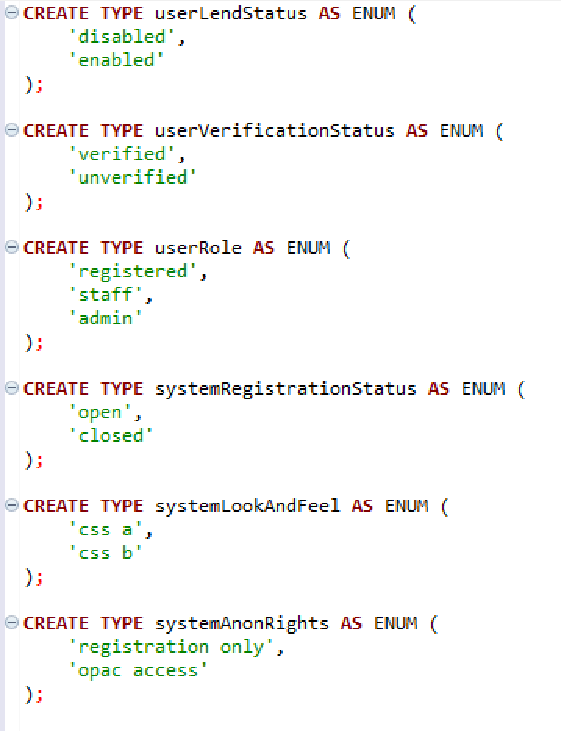
\includegraphics[width=9cm]{SQLENUMs1}
\caption{Die systemeigenen \texttt{ENUM}-Typen}
\end{figure}

\begin{figure}
\centering
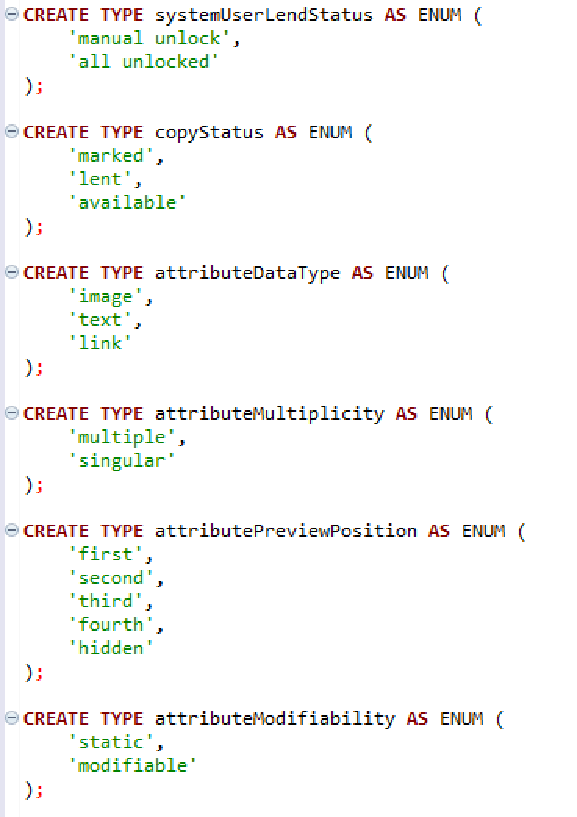
\includegraphics[width=9cm]{SQLENUMs2}
\caption{Weitere \texttt{ENUM}-Typen}
\end{figure}

\begin{figure}
\hypertarget{User}{}
\flushleft
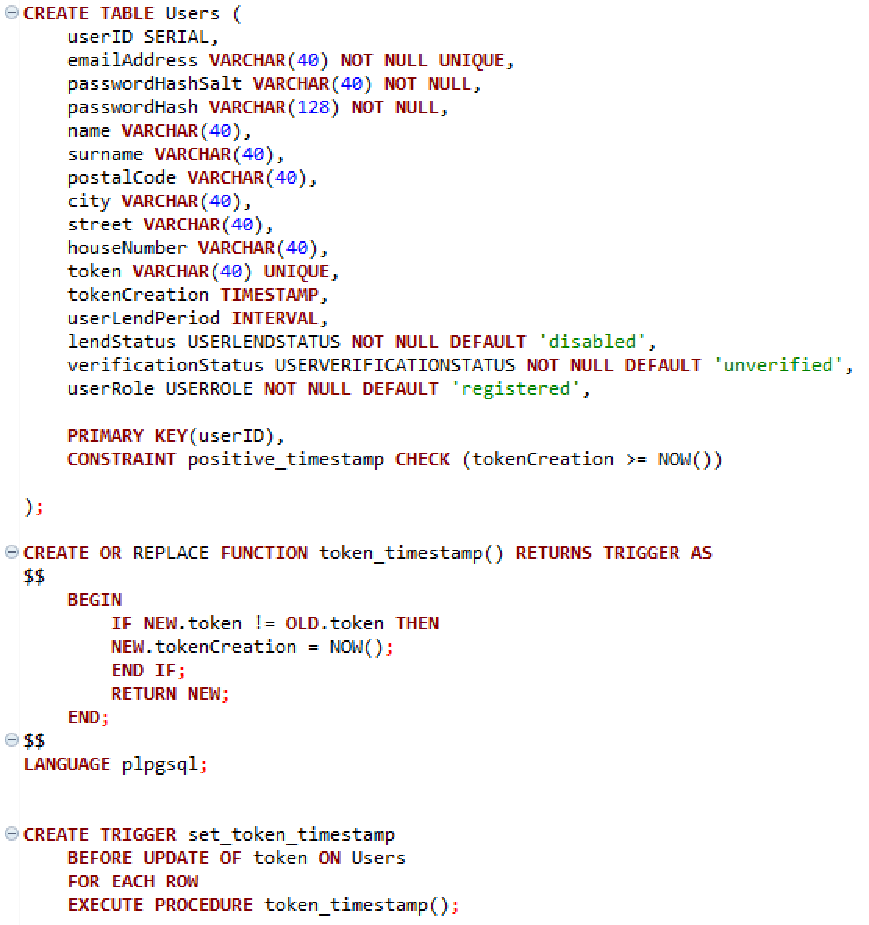
\includegraphics[width=50em]{SQLUSER}
\caption{SQL-Anweisung zum Erstellen der Nutzertabelle, mit automatischem Setzen der Tokenerstellzeit.}
\end{figure}

\begin{figure}
\hypertarget{Medium}{}
\flushleft
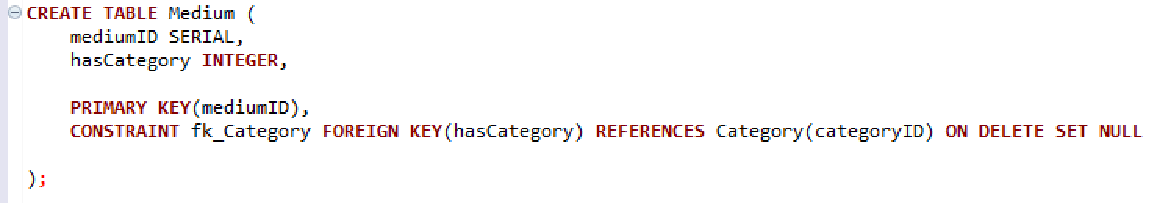
\includegraphics[width=60em]{SQLMEDIUM}
\caption{SQL-Anweisung zum Erstellen der 'Medium'-Tabelle.}
\end{figure}

\begin{figure}
\hypertarget{Application}{}
\flushleft
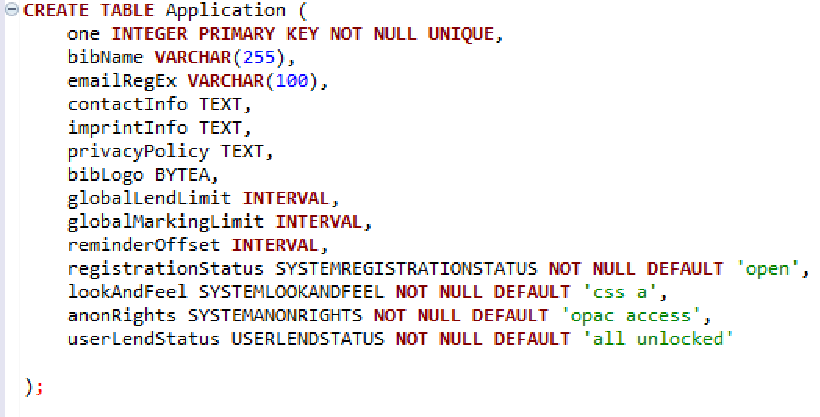
\includegraphics[width=45em]{SQLAPPLICATION}
\caption{SQL-Anweisung zum Erstellen der 'Applikations'-Tabelle. Hier werden Anwendungseinstellungen gespeichert.}
\end{figure}

\begin{figure}
\hypertarget{Category}{}
\flushleft
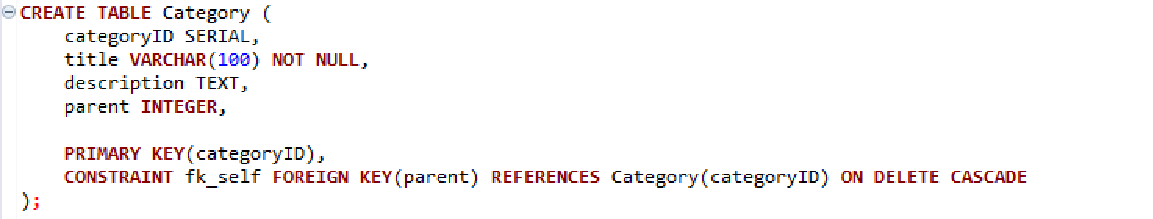
\includegraphics[width=60em]{SQLCATEGORY}
\caption{SQL-Anweisung zum Erstellen der 'Kategorie'-Tabelle.}
\end{figure}

\begin{figure}
\hypertarget{CustomAttribut}{}
\flushleft
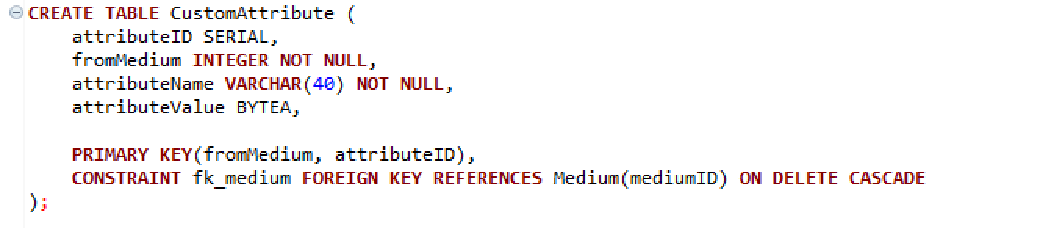
\includegraphics[width=60em]{SQLCUSTOMATTRIBUTE}
\caption{SQL-Anweisung zum Erstellen der 'Attribute'-Tabelle.}
\end{figure}

\begin{figure}
\hypertarget{AttributeType}{}
\flushleft
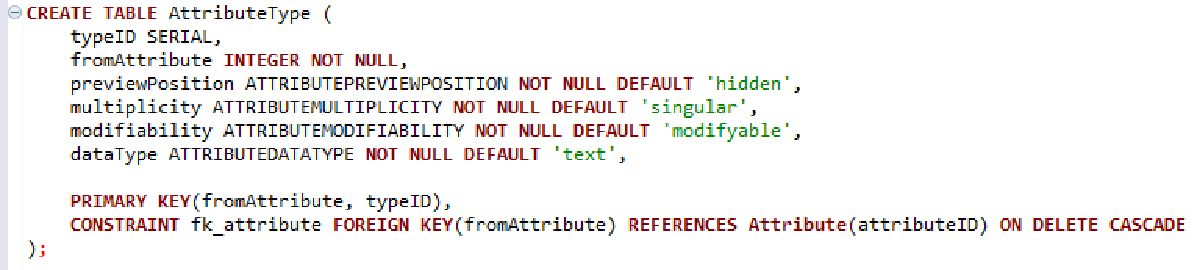
\includegraphics[width=60em]{SQLATTRIBUTETYPE}
\caption{SQL-Anweisung zum Erstellen der Tabelle für Attributtypen.}
\end{figure}

\begin{figure}
\hypertarget{Copy}{}
\centering
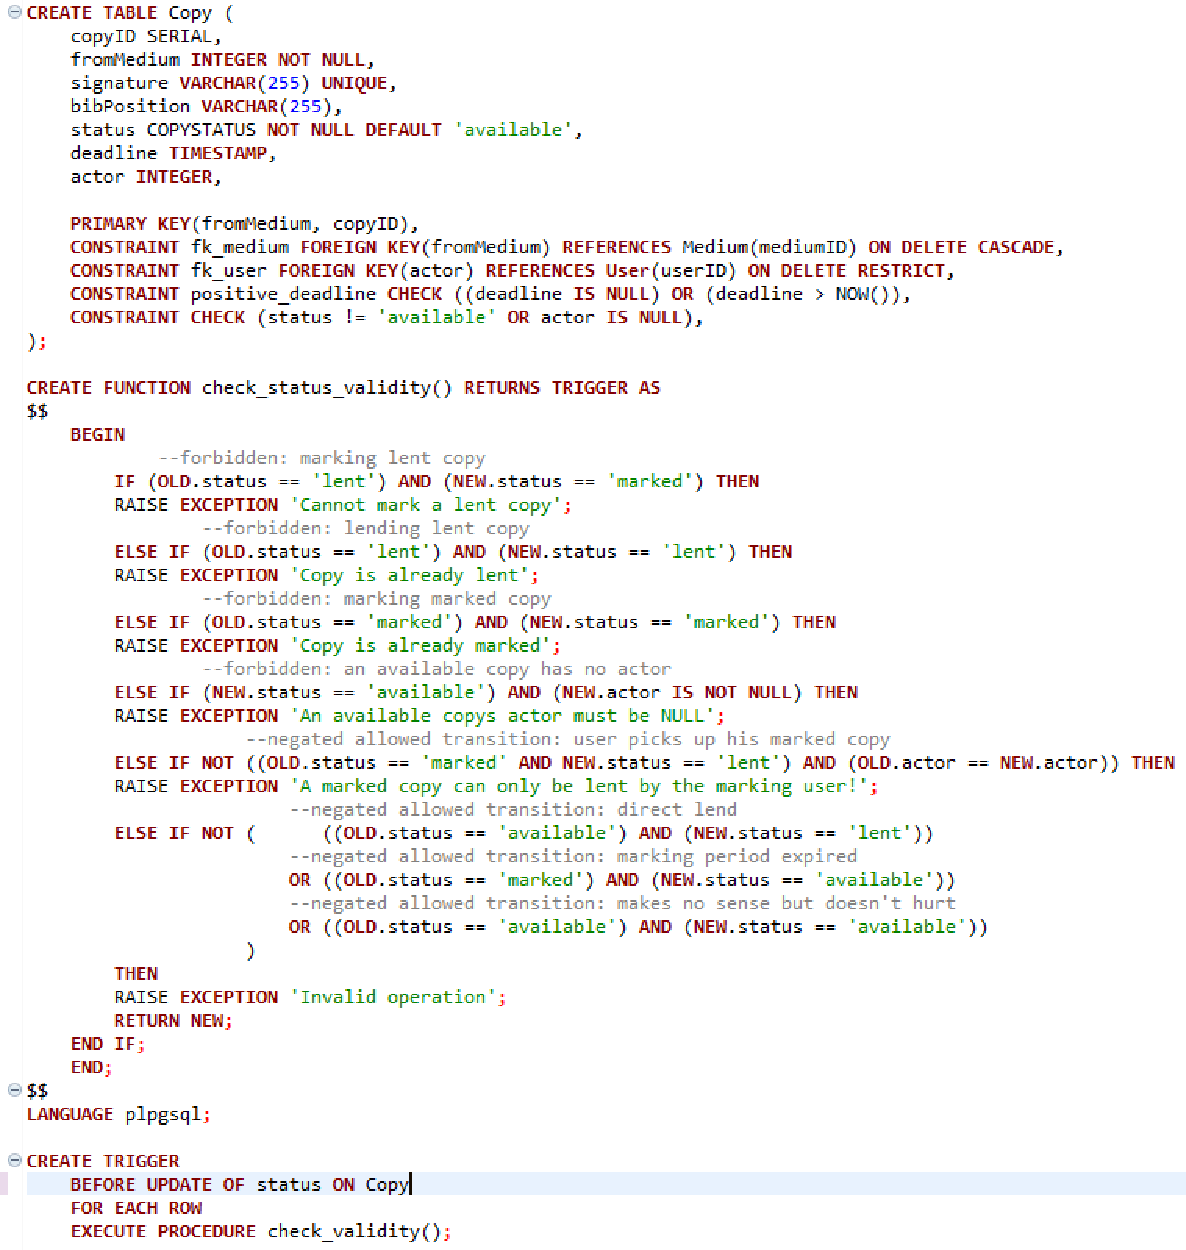
\includegraphics[width=60em]{SQLCOPY}
\caption{SQL-Anweisung zum Erstellen der 'Exemplar'-Tabelle mit Integritätschecks für die 'ausgeliehen'- und  'markiert'-Relationen.}
\end{figure}
\restoregeometry

\subsection{Normalformanalyse}
Zunächst werden die erstellten Tabellen in klassischer Notation für Relationen aufgelistet: \\
\\
\textbf{User}:\{ \textit{userID, emailAddress, passwordHashSalt, passwordHash, name, surname, postalCode, city, street, houseNumber, token, tokenCreation, userLendPeriod, lendStatus, verificationStatus,\\ userRole} \}\\
\textbf{Medium}:\{ \textit{mediumID, hasCategory} \}\\
\textbf{Application}:\{ \textit{one, bibName, emailRegEx, contactInfo, imprintInfo, privacyPolicy, bibLogo, globalLendLimit, globalMarkingLimit, reminderOffset, registrationStatus, lookAndFeel, anonRights,\\ userLendStatus} \}\\
\textbf{Category}:\{ \textit{categoryID, title, description, parent} \}\\
\textbf{CustomAttribute}:\{ \textit{attributeID, fromMedium, attributeName, attributeValue} \}\\
\textbf{AttributeType}:\{ \textit{typeID, fromAttribute, previewPosition, multiplicity, modifiability, dataType} \}\\
\textbf{Copy}:\{ \textit{copyID, fromMedium, signature, bibPosition, status, deadline, actor} \}\\
\\
Aus den funktionalen Abhängigkeiten zwischen den Attributen ergeben sich verschiedene Superschlüssel für die Relationen. Die Superschlüsselmöglichkeiten sind eingeklammert.\\
\\
\textbf{User}:\{ (\texttt{userID}), (\texttt{emailAddress}), (\texttt{token}), (\texttt{userID, token}), (\texttt{userID, emailAddress}), \\ (\texttt{emailAddress, token}), (\texttt{userID, emailAddress, token}), \textit{passwordHashSalt, passwordHash, name, surname, postalCode, city, street, houseNumber, tokenCreation, userLendPeriod, lendStatus, verificationStatus, userRole} \}
Es gibt sowohl Städte mit mehreren Postleitzahlen, als auch Postleitzahlen, die mehrere Städte/Dörfer einschließen. Somit legen sich die Attributwerte nicht gegenseitig eindeutig fest und es besteht keine funktionale Abhängigkeit.\\
\textbf{Medium}:\{ (\texttt{mediumID}), \textit{hasCategory} \}\\
\textbf{Application}:\{ (\texttt{one}),\textit{ bibName, emailRegEx, contactInfo, imprintInfo, privacyPolicy, bibLogo, globalLendLimit, globalMarkingLimit, reminderOffset, registrationStatus, lookAndFeel, anonRights,\\ userLendStatus} \}\\
\textbf{Category}:\{ (\texttt{categoryID}), \textit{title, description, parent} \}\\
\textbf{CustomAttribute}:\{ (\texttt{fromMedium, attributeID}),  \textit{attributeValue, attributeName} \}\\
\textbf{AttributeType}:\{ (\texttt{fromAttribute, typeID}), \textit{previewPosition, multiplicity, modifiability, dataType} \}\\
\textbf{Copy}:\{ (\texttt{fromMedium, copyID}), (\texttt{fromMedium, signature}), (\texttt{fromMedium, signature, copyID}), \textit{bibPosition, status, deadline, actor} \}
Die Attribute \textit{status, deadline, actor} beeinflussen sich gegenseitig, \textit{deadline} hängt jedoch noch von anderen Limits außerhalb dieser Relation ab und wird somit nicht eindeutig durch Änderungen von \textit{actor} oder \textit{status} festgelegt. Da nur der Status 'available' den Wert \texttt{NULL} im Attribut \textit{actor} impliziert und alle anderen Werte keine eindeutige Zuordnung festlegen, gibt es hier keine schlüsselunabhängigen Abhängigkeiten.\\
\\
Aus den minimalen Superschlüssel ergeben sich die Kandidatenschlüsselmöglichkeiten. Da alle Attributewerte nur atomare Werte annehmen können, ist das Schema in erster Normalform. Da es ebenfalls kein nichtprimes\footnote{Ein Attribut, welches nicht Teil eines Kandidatenschlüssels ist.} Attribut gibt, welches von einer echten Teilmenge eines Schlüssel funktional abhängig ist, gilt für das Schema die zweite Normalform. Für jede funktionale Abhängigkeit \textit{X $\rightarrow$ A} gilt außerdem: Entweder ist \textit{A} prim oder\textit{X} ist ein Superschlüssel der Relation. Damit folgt die dritte Normalform. Ohne schlüsselunabhängige Abhängigkeiten bleiben zur Untersuchung nur noch Attribute der überlappenden Kandidatenschlüssel übrig. In keine Richtung bestehen weder zwischen \textit{userID $\leftrightarrow$ token}, \textit{emailAddress $\leftrightarrow$ token} oder \textit{emailAddress $\leftrightarrow$ userID} noch zwischen \textit{signature $\leftrightarrow$ copyID} funktionale Zusammenhänge. Das Relationenschema ist somit in Boyce-Codd-Normalform, da alle Abhängigkeiten von Superschlüsseln ausgehen.



%----------------------------------------------------------------------Kapitel 8--------------------------------------------------------------------------------------------
\newpage
\section{Datenfluss}
\sectionauthor{Sergei Pravdin}
Die Kommunikation zwischen den Klassen und die Interaktionen des Systems werden durch die Sequenzdiagramme abgebildet. Um einen Datenfluss beispielhaft zu zeigen, werden die folgenden beiden Szenarien vorgelegt: Zuerst bucht ein angemeldeter Nutzer ein Medium-Exemplar erfolgreich zur Ausleihe. Im zweiten Szenario bucht ein angemeldeter Nutzer ein Medium-Exemplar erfolglos zur Ausleihe, weil die Verbindung mit der Datenbank fehlgeschlagen ist. Das System ist so eingestellt, dass die angemeldeten Nutzer Zugriff auf die Medien haben. Der Nutzer möchte ein Exemplar des Mediums 'Programmieren lernen' buchen. Im System existiert das Medium mit dem Titel 'Programmieren lernen' und mit der Signatur (ID) '17RE'. Das Exemplar mit der Signatur (ID) '17RE (+1)' gehört zu dem genannten Medium und ist für eine Buchung verfügbar. Der Nutzer ruft die Mediumsseite 'medium.xhtml?id=17RE' auf.
\subsection{Interaktionen beim erfolgreichen Buchen eines Medium-Exemplars}
\subsubsection{Initialisierung der Mediumsseite}
Beim Laden der Mediumsseite wird zuerst die Methode 'init' als @PostConstruct aufgerufen. Die 'init'-Methode erzeugt ein Medium-DTO, das Medium-DTO hat eine Kollektion der CopyDTOs und eine Kollektion der AttributeDTOs, folglich werden sie vom Medium-DTO erstellt. Der Nutzer bekommt das MediumDTO und setzt eine Medium-ID, die aus dem 'viewParam' zur Verfügung gestellt wird. Danach wird die 'viewAction()' durchgeführt, welche die Mediumsseite durch die statische Methode aus dem Medium-DAO liefern muss. Das Medium-DAO bekommt auf der Persistence-Schicht eine Verbindung von der Singleton-ConnectionPool-Klasse durch die Methoden 'getInstance()' und 'getConnection()'. Im Körper der Methode 'loadMedium' wird eine SELECT-Anfrage durchgeführt, danach gibt das Medium-DAO die Verbindung durch die Methode 'releaseConnection' frei. Das Medium-DAO befüllt mit den von der Datenbank erhaltenen Attributen das Medium-DTO (inkl. CopyDTOs und AttributeDTOs) und gibt es dem Medium-BB zurück. Die Mediumsseite ist nun durch die Methode 'getAttributes' des Medium-DTOs vollständig geladen.
\subsubsection{Buchen eines Exemplars}
Durch die Methode 'getCopies' des Medium-DTOs ist das gewünschte Exemplar für den Nutzer sichtbar. Der Nutzer klickt auf den Buchen-Button des Exemplars. Beim Klicken ruft der Nutzer die Methode 'pickUpAnyCopy' des Medium-BBs auf. Im Körper dieser Methode wird die Methode 'checkAccountStatus()' aus dem UserSession-BB aufgerufen, um zu prüfen, ob der Nutzer Zugriff auf die Funktion Buchen hat. Das UserSession-Bean meldet dem Medium-BB ein positives Ergebnis (OPENED-Status) zurück. Das Medium-BB ruft die statische Methode 'MediumDAO.pickUpAnyCopy(mediumDTO)' auf. Das Medium-DAO bekommt durch die Methoden 'getInstance()' und 'getConnection()' auf der Persistence-Schicht eine Verbindung von der Singleton-ConnectionPool-Klasse. Falls ein availabilityStatus des Exemplars immer noch 'AVAILABLE' ist, wird wird eine UPDATE-Anfrage im Körper der Methode 'loadMedium'  durchgeführt. Im Anschluss gibt das Medium-DAO die Verbindung durch die Methode 'releaseConnection' frei. Als Ergebnis der Methode 'pickUpAnyCopy' bekommt das Medium-BB 'true'. Das Medium-BB vergibt den neuen Status 'MARKEDTOCOLLECT' an das Exemplar. Der Nutzer bekommt eine Nachricht durch die statische Methode 'RessourceBandleHandler.getValue()' und die Buchung ist erfolgreich abgeschlossen. Vom Ressource-Bandle-Handler wird der Nutzer entsprechend benachrichtigt.
\newgeometry{left=0cm,right=0cm,top=0cm,bottom=2cm}
\newpage
\begin{figure}[h]
    \centering
    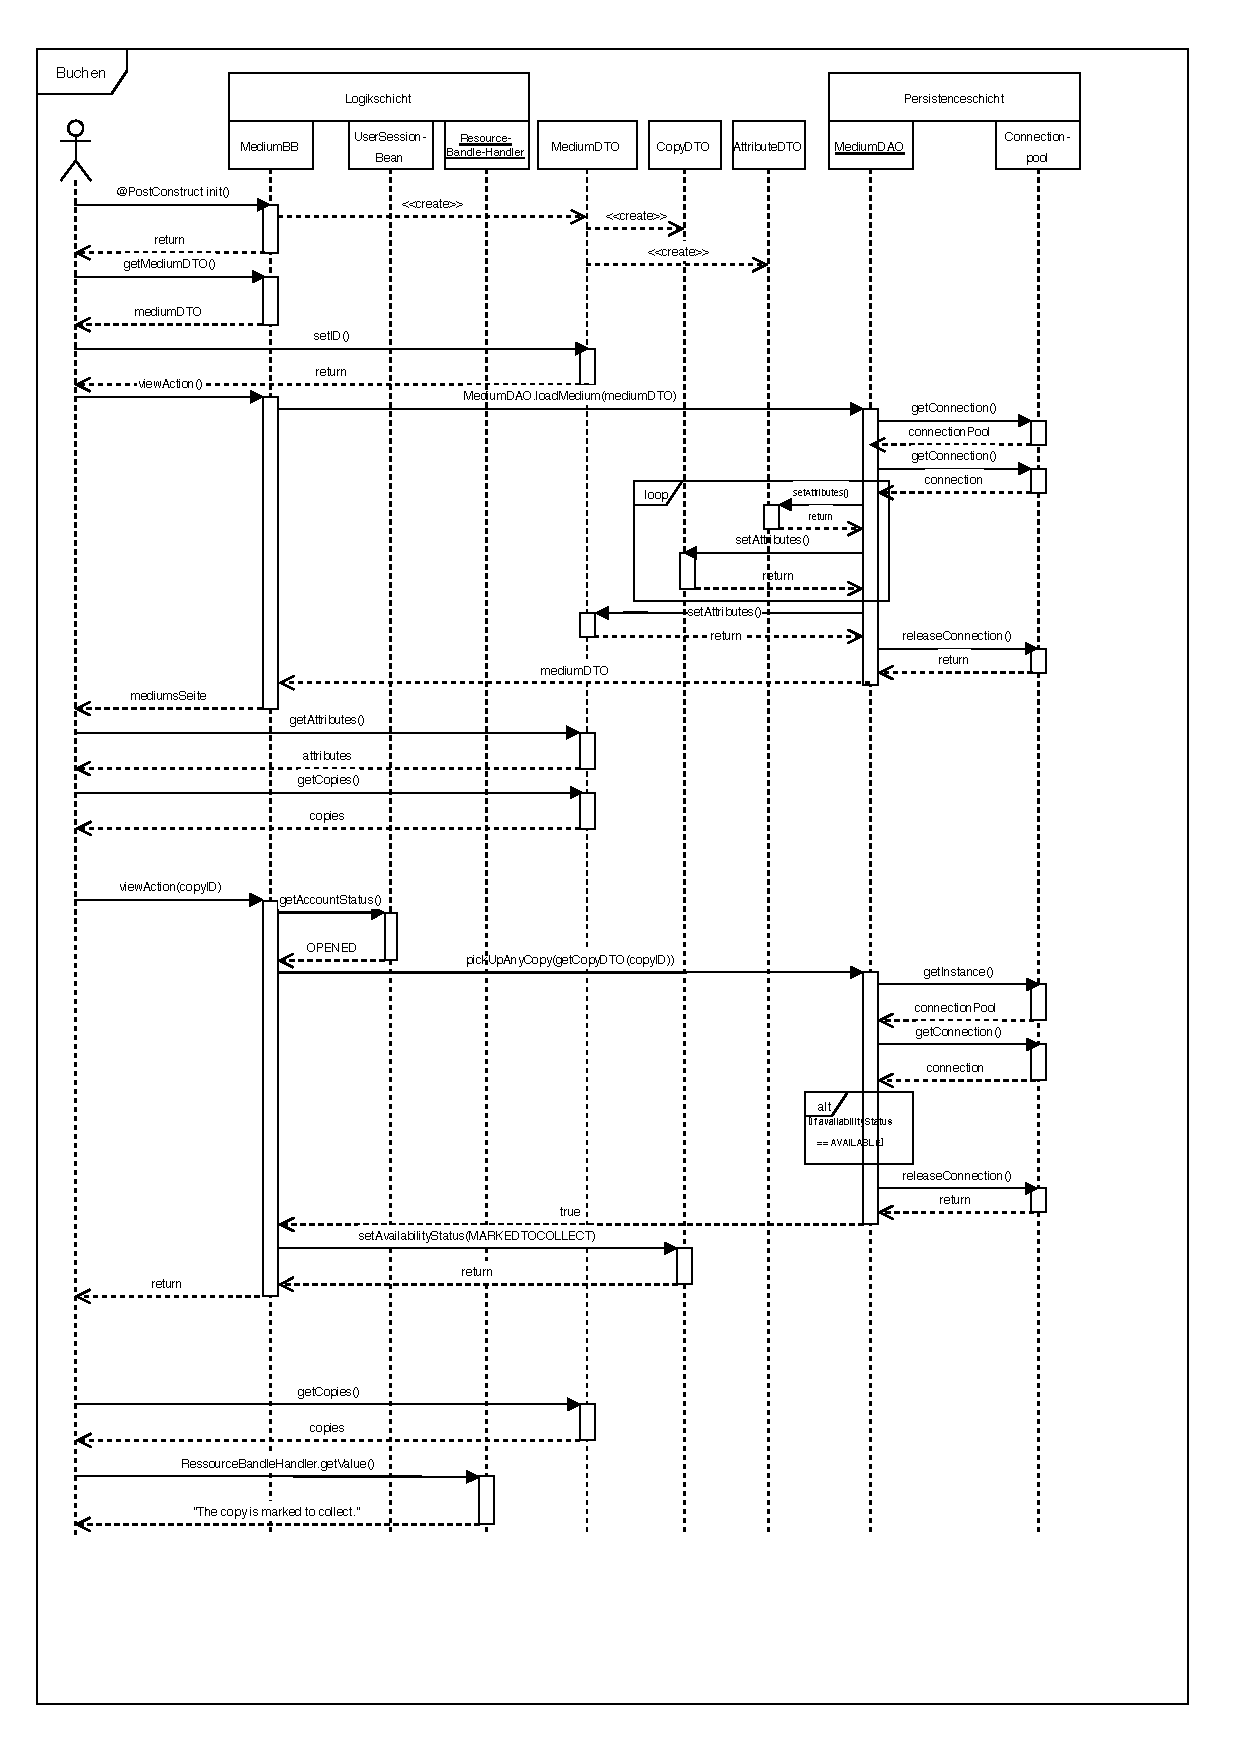
\includegraphics[width = 50em]{Sequenzdiagramm-success-v3.2}
    \caption{Interaktionen beim erfolgreichen Buchen eines Medium-Exemplars}
    \label{Sequenzdiagramm}
\end{figure}
\restoregeometry

\subsection{Interaktionen beim Buchen eines Medium-Exemplars mit fehlender Datenbankverbindung}
\subsubsection{Initialisierung der Mediumsseite}
Beim Laden der Mediumsseite wird zuerst die Methode 'init' als @PostConstruct aufgerufen. Die 'init'-Methode erzeugt ein Medium-DTO, das Medium-DTO hat eine Kollektion der CopyDTOs und eine Kollektion der AttributeDTOs, folglich werden sie vom Medium-DTO erstellt. Der Nutzer bekommt das MediumDTO und setzt eine Medium-ID, die aus dem 'viewParam' zur Verfügung gestellt wird. Danach wird die 'viewAction()' durchgeführt, welche die Mediumsseite durch die statische Methode aus dem Medium-DAO liefern muss. Das Medium-DAO bekommt durch die Methoden 'getInstance()' und 'getConnection()' auf der Persistence-Schicht eine Verbindung von der Singleton-ConnectionPool-Klasse. Aufgrund der fehlenden Verbindung mit der Datenbank kann das Medium-DAO keine SELECT-Anfrage durchführen, deshalb bekommt das Medium-DAO einen SQL-Exception. Das Medium-DAO wandelt den SQL-Exception in den DataAccess-Exception um, danach gibt das Medium-DAO eine Verbindung durch die Methode 'releaseConnection' frei. Im nächsten Schritt wirft das MediumDAO einen Data-Access-Exception in den Medium-BB ein. Der Nutzer ruft die Methode 'handle' des ExceptionHandlers auf; der ExceptionHandler gibt den Fehler durch die Methoden 'getInstance()' und 'addValue(Data-Access-Exception)' in die Singleton-Logger-Klasse ein. Danach bekommt der ExceptionHandler eine Message vom Resource-Bandle-Handler und setzt diese Message in die ErrorBB-Klasse ein.
\subsubsection{Weiterleitung zur Fehlerseite}
Als Ergebnis der Methode 'handle' liefert der ExceptionHandler dem Nutzer den Link zur Fehlerseite. Das Laden der Fehlerseite wird auf dem Sequenzdiagramm nicht abgebildet.

\newpage

\newgeometry{left=0cm,right=0cm,top=0cm,bottom=2cm}

\begin{figure}[h]
	\hypertarget{Fehlersequenz}{}
    \centering
    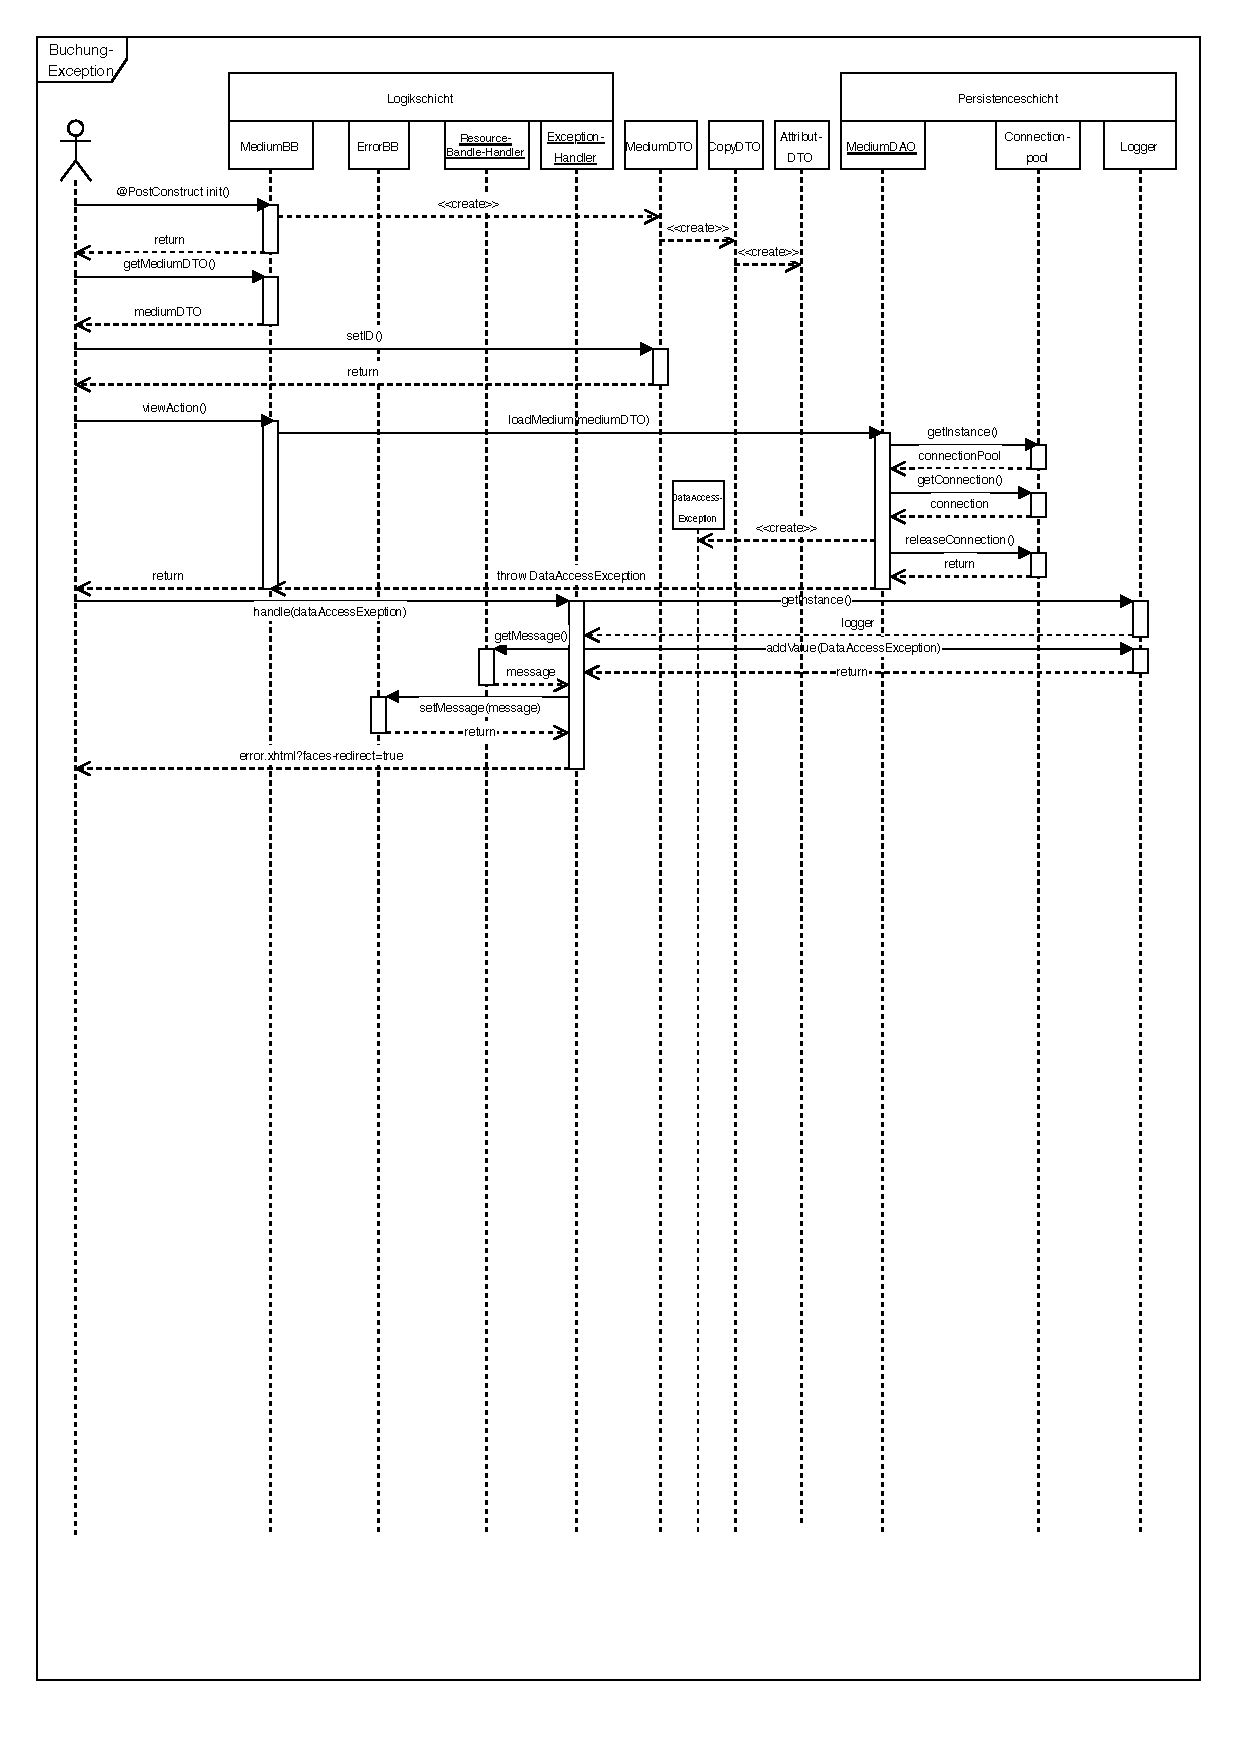
\includegraphics[width = 50em]{Sequenzdiagramm-exception-v4.1}
    \caption{Interaktionen beim Buchen eines Medium-Exemplars mit fehlender Datenbankverbindung}
    \label{Sequenzdiagramm}
\end{figure}

\restoregeometry
\newpage

%----------------------------------------------------------------------Kapitel 9--------------------------------------------------------------------------------------------
\section{Sicherheit}
Dieses Kapitel baut auf dem Abschnitt 'technische Systemsicherheit' des Entwurfs auf und vertieft Sicherheitsaspekte der Anwendung.
\subsection{Injections}
\hypertarget{Injections}{Das} direkte Interpretieren von nutzergenerierten Eingaben wird unterbunden.\\
\textbf{SQL:} Da unser System postgreSQL als Datenbankanfragesprache verwendet, wird in den \hyperlink{DAOs}{Data Access Objects} im Java-Code mit \hyperlink{https://docs.oracle.com/javase/7/docs/api/java/sql/PreparedStatement.html}{'PreparedStatements'} gearbeitet. Da die eigentliche Anfrage nicht zusammen mit den vom Nutzer stammenden Parametern interpretiert wird, hat das Einschleusen von SQL-Code in diese Parameter keinen Effekt auf die Datenbank.\\
\textbf{HTML/JavaScript:} \hypertarget{XSS}{Um} das Einschleusen von HTML- (und eingebetteten JavaScript-) Code, in nutzergenerierte Inhalte der Webseite zu verhindern, verfügen die JSF-Facelet Elemente für User-Inputs über integrierte Escaping-Funktionen. Alle nutzergenerierten Anzeigen der Webseite werden so direkt am Input geschützt.
\subsection{Insecure Direct Object References}
Unbefugte direkte Zugriffe auf zugangsbeschränkte Teile der Anwendung werden abgefangen.\\
Nutzer könnten versuchen, manuell die URL-Parameter in der Adresszeile zu verändern. In der Medienansicht könnte man so z.B. durch Ändern der ID auf die Ansicht eines anderen Mediums gelangen. Bei einer Anfrage werden erste Maßnahmen der Zugriffskontrolle nach der \texttt{RESTORE\_VIEW}-Phase im \hyperlink{PhaseListener}{Trespasslistener} vorgenommen. Hier wird über die Sessionmap die Nutzerrolle und der Loginstatus mit der URL-Struktur der Anfrage abgeglichen und bei invalidem Zugriff entsprechend umgeleitet. Um denselben Zugriffsprozess wie im Mediumsansicht-Beispiel bei der Profilseite zu verhindern, wird im Backing-Bean durch Zugriff auf die URL-Parameter geprüft, ob der Nutzer berechtigt ist, andere Profile als sein eigenes anzusehen.
\subsection{Session Fixation}
Wie bereits im Abschnitt 'Session-Hijacking' des Entwurfs erwähnt, tauschen wir unmittelbar nach dem Login eines Benutzers im \hyperlink{Login}{Backing-Bean} den Identifikator der Nutzer-Session aus. \hyperlink{Session}{UserSession}-Objekte werden nur für eingeloggte Nutzer angelegt und beim Login werden keine vorherigen Zustandsinformationen übernommen.  Zusätzlich zur Zerstörung beim Logout haben alle Sessions Tomcat-intern einen Inaktivitätstimeout von 30 Minuten, den wir beibehalten werden (andere Servlet Container verwenden denselben Timeout).
\subsection{Userinput}
Neben dem Vorbeugen von \hyperlink{Injections}{Injections} gibt es weitere Maßnahmen zum Absichern von Nutzereingaben.\\
\textbf{Admins:} Ausnahmen von den \hyperlink{XSS}{XSS-Gegenmaßnahmen} bilden das Impressum, die Datenschutzerklärung und  die Kontaktinformationen, da wir Administratoren beim editieren mehr Gestaltungsmöglichkeiten geben wollen. Andere Nutzerrollen haben keinen schreibenden Zugriff auf diese Teile der Webseite.\\
\textbf{Passwörter:} Eine Mindestlänge von 8 Zeichen in Groß- und Kleinschreibung und das enthalten einer Zahl wird durch den \hyperlink{Validator}{PasswordValidator} sichergestellt. Registrierte Passwörter werden nicht im Klartext gespeichert, sondern in der Klasse \hyperlink{Hash}{PasswordHashingModule} durch eine Hashfunktion geschickt. Durch vorheriges Anhängen eines Salts\footnote{Ein kurzer, zufällig generierter String.} an das Passwort werden Kollisionen der Hashfunktion unwahrscheinlicher und gleiche Passwörter entsprechen nicht mehr demselben Hashwert.\\
\textbf{E-Mail-Adressen:} Bei der Registrierung eines neuen Nutzerkontos oder der Änderung der Adresse wird der vom Administrator festgelegte RegEx zuerst bedient und danach wird auf Duplikate in der Datenbank geprüft. Dies geschieht im \hyperlink{Validator}{EmailValidator}. Der anschließende Verifizierungsprozess stellt die Gültigkeit der Adresse sicher.
\subsection{System Secrecy}
Die Hintergrundprozesse und Technologien werden bestmöglich versteckt.\\
\textbf{Rollenisolation:} Ist der Nutzer berechtigt, das unter der URL erreichbare Facelet zu sehen, werden, anhand der Nutzerrolle,vorhandene Knöpfe und Eingabefelder je nach Rollenberechtigungen gerendert oder ausgeblendet. So haben Rollen der unteren Hierarchieschichten keine Information über die Möglichkeiten der darüber liegenden.\\
\textbf{Technologiemaskierung:} Der XML-Dialekt der Facelet-Sprache ist für den Benutzer undurchsichtig, die Sprache wird durch das Framework in HTML und JavaScript mit der Endung '.xhtml' umgewandelt. Weder das verwendete Datenbanksystem noch das JSF-Framework sind für den Benutzer ersichtlich. Im laufenden System werden bei Fehlermeldungen eigene Fehlerseiten erstellt und keine Stack-Traces ausgegeben, um die Tomcat-eigenen Fehlerseiten nicht preiszugeben. Wenn möglich wird, durch die vorgezogene Verwendung von \textit{Forwards} statt \textit{Redirects} bei der Seitennavigation die URL gleich bleiben und dadurch die interne Ordnerstruktur zumindest teilweise maskiert.

\end{document}
